\chapter{Preliminary Work}\label{C:preliminary}

This chapter presents the highlights of the initial work conducted on the creation of a Web service composition approach that combines a planning algorithm, for candidate creation and modification, with EC techniques, for optimising candidates according to their overall Quality of Service. In particular, two types of direct solution representations are explored, in alignment with Objective \ref{obj:rep}: a \textit{tree-based representation}, which is compatible with the existing Genetic Programming algorithm but may lead to service duplication problems, and a \textit{graph-based representation}, which prevents duplication issues but requires a more complex evolutionary algorithm. These two approaches are discussed and compared in the following sections.

\section{Motivation}
\section{Motivation and Problem Description}\label{Motivation and Problem Description}
\subsection{Motivation}\label{Motivation}

The aim of web service composition considered in this paper is to automatically compose optimal solutions in considering both QoS and semantic matchmaking quality based on a user's request. The request is to provide inputs and obtain outputs. The resulting composition of this request is a composition solution with an optimal comprehensive quality in terms of semantic matchmaking quality and QoS. A motivating example of this problem is shown in Fig \ref{motivation}. The figure shows a DAG that represents a solution with four web services involved for a request $R$ as a composition task, where inputs of the task are \{$TravelDepartureDate$, $HomeCity$, $ConferenceCity$, $TravelReturnDate$ \} and outputs are \{$BusTicket$, $FlightTicket$, $TouristMap$, $HotelReservation$ \}. This is a classic example of travel planning problem for people who seek for booking services of airplanes, buses and hotels reservation, and also generating tourist maps for the conference city. The graph also contains edges that marked with connected outputs and inputs of two connected atomic services, which represent valid semantic matches that the outputs of a web service can be passed as the inputs of its successors.

\begin{figure}[h]
\centering
\fbox{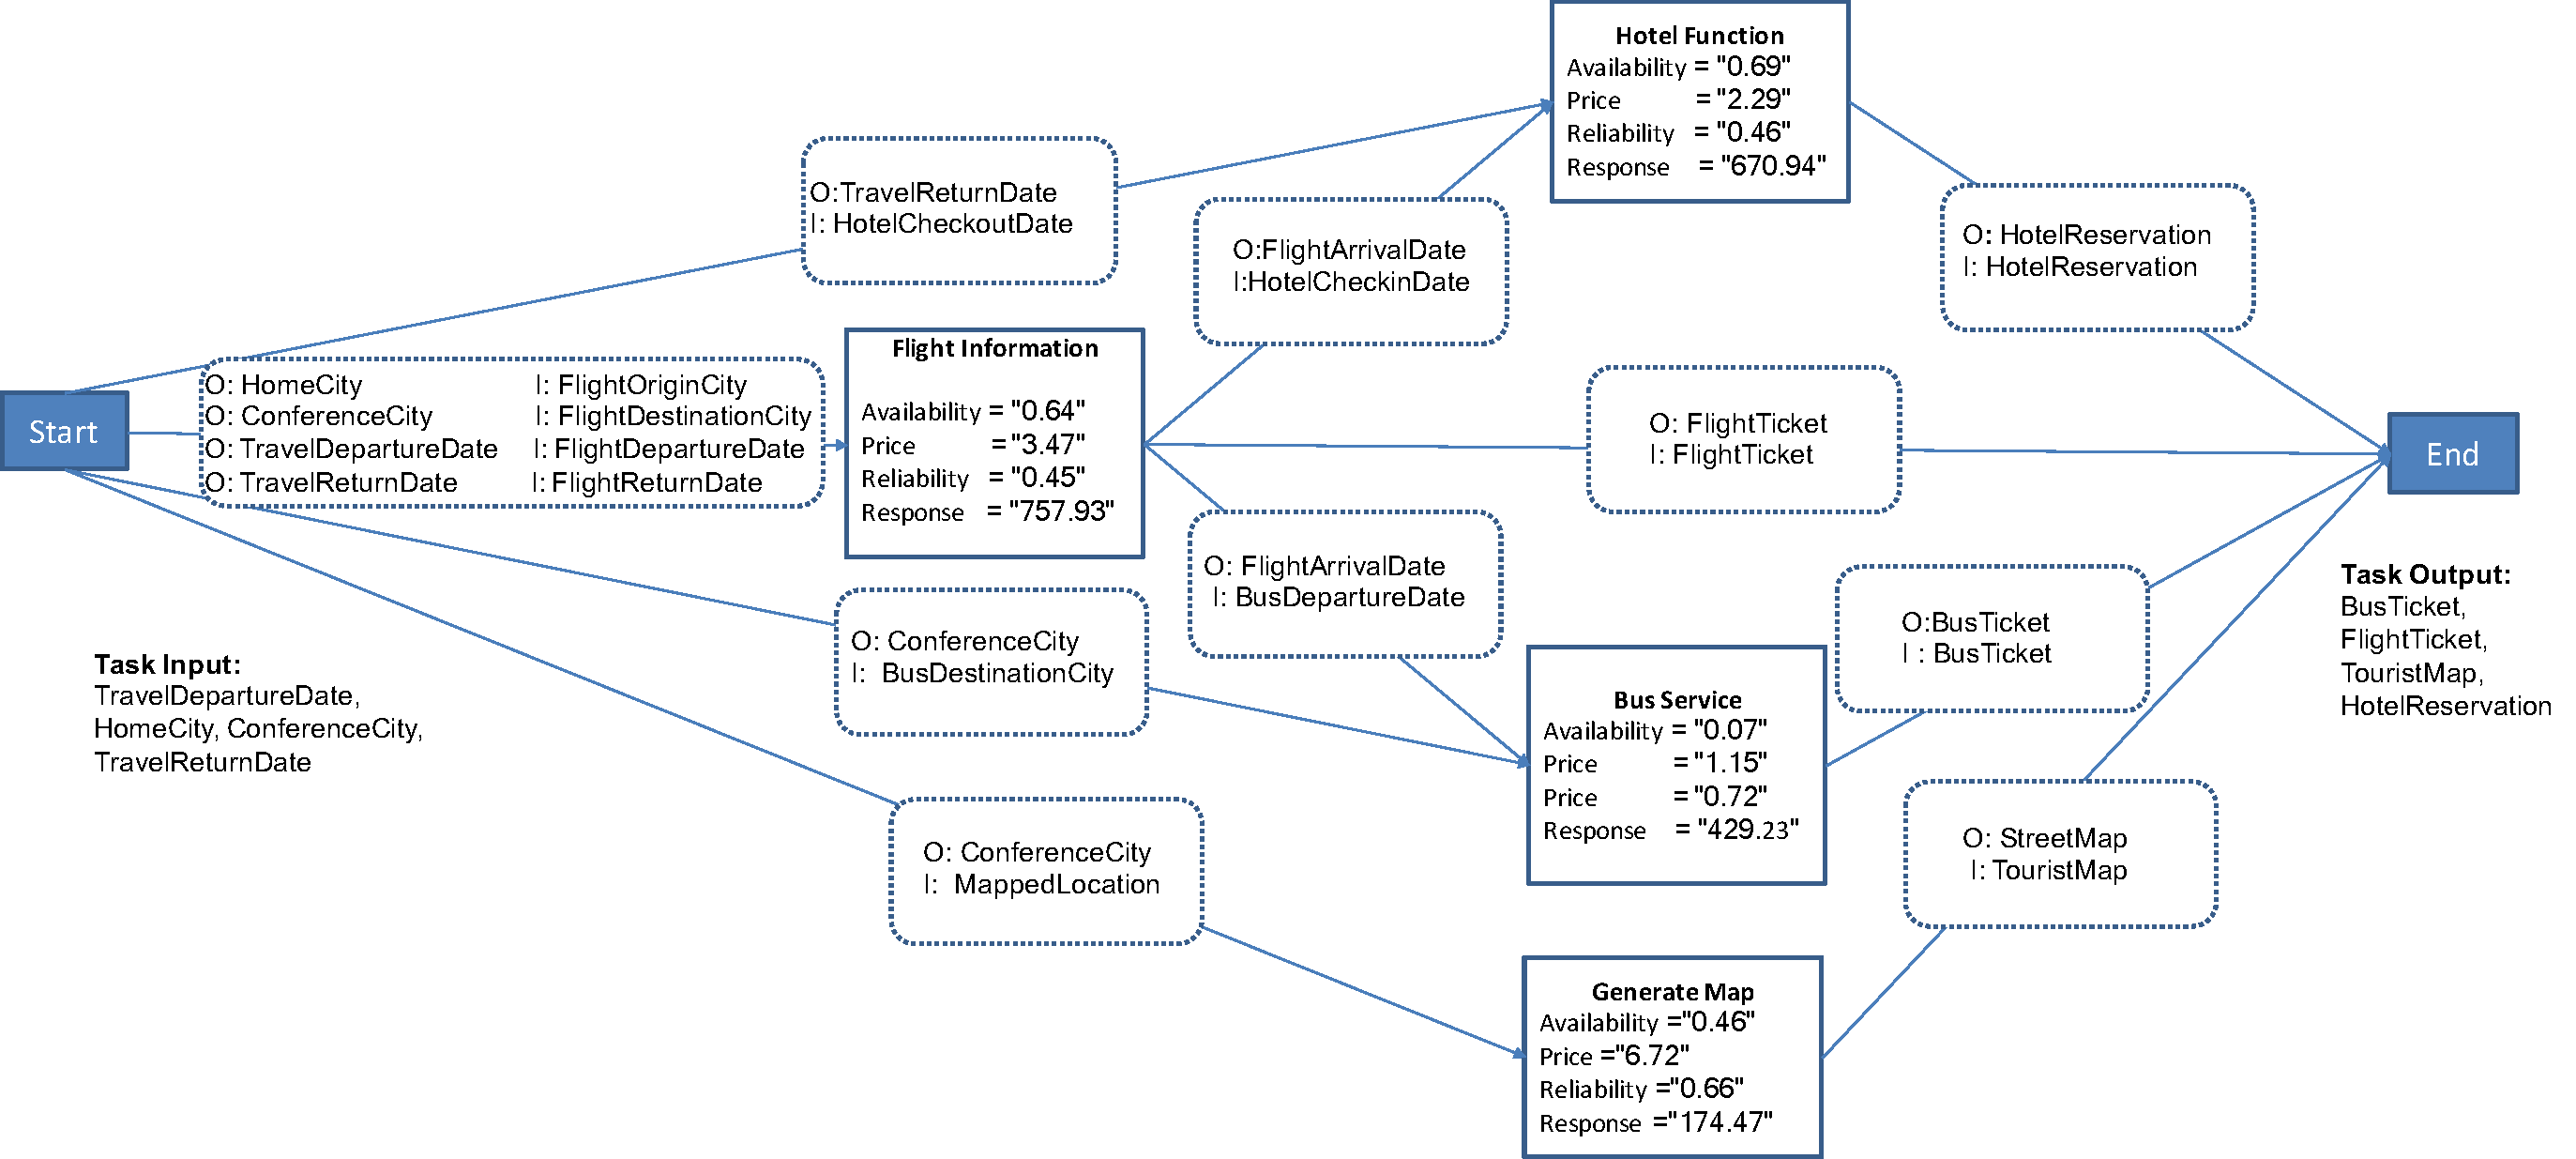
\includegraphics[scale=.25]{motivation.pdf}}
 \caption{ An example of a web service composition}
 \label{motivation}
\end{figure}

Although obtaining a correct combination of web service is essential, there are many ways to connect multiple web services chosen from a service repository. These web services provide different QoS in terms of availability, price, reliability and response time. Moreover, valid semantic matches between two connected web services could also have different matchmaking quality. For example, $Generate Map$ service produce $StreetMap$ which is considered to be a valid semantic match to $TouristMap$, but $Bus Service$ produce $BusTicket$ which is considered to be a better valid semantic match to $BusTicket$. The descriptions of these matched resources are captured in a ontology depicted in Fig .\ref{taxonomy}, where all the inputs and the outputs related to the web services are described for the travel planning problem discuss here. For example, the concept $Map$ and its sub-concept $urbanMap$ are assigned with a $touristMap$ instance and $streetMap$ instance respectively in Fig .\ref{taxonomy}. The valid semantic match is considered that an instance of $urban Map$ can be an instance of $Map$, but not vice versa. To demonstrate the motivation of proposing a comprehensive quality, we give a simple example here. The service $GenerateMap$ with a output ($StreetMap$) and a price (``6.72") in the web service composition can be replace by a service $GenerateTouristMap$ with a different output ($TouristMap$) and a different price (``16.87") available in the service repository. This composition solution results in a better semantic matchmaking quality, but price negatively contributes to the QoS. Therefore, to reach the optimal solutions automatically, we need to measure these changes to the solutions considering matchmaking quality and QoS simultaneously. 



\begin{figure}[h]
\centering
\fbox{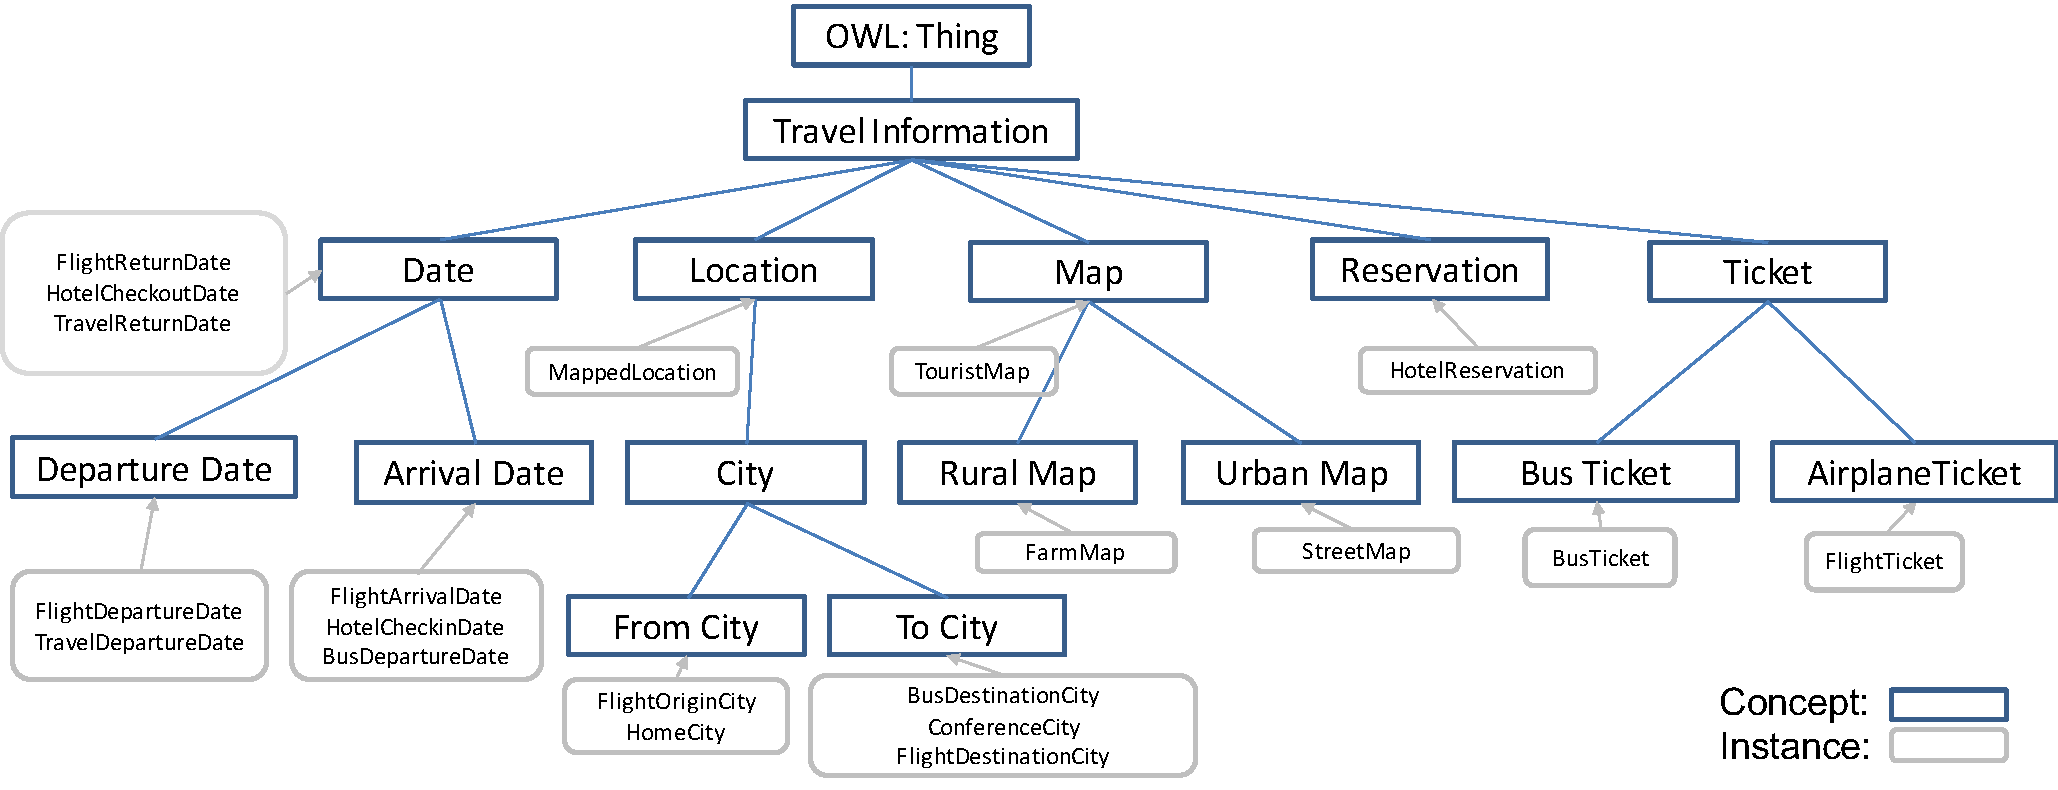
\includegraphics[scale=.28]{taxonomy.pdf}}
 \caption{ An ontology of a travel planning domain}
 \label{taxonomy}
\end{figure}



\section{Problem Formalisation}

More formally, a Web service composition that includes conditional constraints can be considered a reachability problem where, given a composition input set $I$, a group of services is assembled in order to produce multiple composition output sets $O_1$ to $O_m$, each output being dependent on a sequence of conditions $C_1$ to $C_n$ that leads to that outcome. Users often expect these services to be optimised according to their quality, giving higher weights to reflect the priority of quality attributes. Based on this understanding, a \textit{composition task} can be represented as a tuple $T = (P, W)$. $P$ is a collection of paths from the provided input $I$, going through some conditions $C$ to reach one of required output possibilities $O_i$, essentially forming a tree $P = \{\langle I,C,O_i\rangle\}$, and \textit{W} is the set of priority weights for each Quality of Service (QoS) attribute. A \textit{Web service} is a tuple $S_x = (I_x, O_x, Q_x)$, where $I_x$ is the set of inputs that must be provided in order to execute the service, $O_x$ is the set of outputs produced by the service after execution, and $Q_x$ are the service's QoS attributes. Finally, a \textit{Web service composition} is a minimal set of paths where all services appearing in a path are sequentially linked, and where interleaved conditional nodes are allowed. Thus, it can be described as $WSC = \{\langle I,(S,C_x)*,S,O_i\rangle\}$. The inputs of all services in the sequences $S$ are fully satisfied if all paths in the composition are considered, and the same is true for the various $O$ possibilities. A property of the paths in $WSC$ is that if all services are removed from a path $a \in WSC$, then its shortened version corresponds to a path in $P$ (i.e. $a_{short} \in P$).

\subsection{Ontology-based Index Cached Optimisation}\label{indexCache}
our PSO-based approach demands decoding processes from optimised queues to weighted DAGs, a bottleneck of efficiently constructing weighted DAGs lie in building required information of edges, which is related to the cost of $fullmatch$
$(a \Rightarrow b)$ identifications and $sim(a, b)$ calculations between input-related and output-related concepts of service candidates. To efficiently construct weighted DAGs, we calculate $sim(a, b)$ of all $fullmatch(a \Rightarrow b)$ interleaving with the greedy search discussed in Sect \ref{PSO_based_approach}. This information is stored in a table structure with special $X$ value if no $fullmatch(a \Rightarrow b)$ is satisfied. Therefore, this optimised cache contributes to less and constant time for weighted DAG building through the evolutionary process.


We utilise benchmark dataset web service challenge 2009 (WSC09) \cite{kona2009wsc} to perform the evaluation. WSC09 provides problems with five tasks corresponding to variable number of services, and ontologies. Therefore, it is a challenge dataset for measuring the scalability of our quality evaluation model. Table \ref{wsc09datasetTable} presents the features of the WSC’09 dataset. The number of concepts, individuals in the ontology and services in each data set is shown in the second, third, fourth column respectively. Also, we extend all the datasets with QoS attributes from service providers to enable our evaluation. 

\begin{table}[]
\centering
\caption{Features of the WSC09 datasets}
\label{wsc09datasetTable}
\begin{tabular}{l|l|l|l}
\hline
\multicolumn{1}{c|}{Dataset} & No.Concept & No.Individual & No.Service \\ \hline
WSC09 01                     & 1578       &3102           &572      \\ \hline
WSC09 02                     & 12388      &24815          &4129      \\ \hline
WSC09 03                     & 18573      &37316          &8138      \\ \hline
WSC09 04                     & 18673      &37324          &8301      \\ \hline
WSC09 05                     & 31044      &62132          &15211    \\ \hline
\end{tabular}
\end{table}

\section{EC-Based Composition Approaches}

Evolutionary Computation (EC), a series of optimisation techniques inspired by Darwin's theory of evolution \cite{back2000evolutionary}, has been successfully employed to solve the problem of automated Web service composition \cite{pejman2012web}. In EC, the general idea is to create a population of candidates, and then gradually improve them through the use of genetic operators to reach an optimised solution several generations later. These operators are usually crossover, where part of the genetic material of two candidates is exchanged at random, and mutation, where part of the genetic material of a candidate is randomly modified; the quality of candidates is measured by a fitness function that rewards desirable characteristics. The advantage of using EC for Web service composition is that it can handle very large numbers of available services, while traditional techniques such as integer programming have been shown to not scale well \cite{canfora2005approach}. The EC-based Web services composition approaches discussed in this chapter share a number of similarities in the way they function, and Algorithm \ref{compSteps} summarises the general procedure followed by both of them.

\begin{algorithm}
 \setlength\hsize{0.9\linewidth}
 \SetKwInOut{Input}{Input}\SetKwInOut{Output}{Output}
 \let\oldnl\nl% Store \nl in \oldnl
\newcommand{\nonl}{\renewcommand{\nl}{\let\nl\oldnl}}
 \LinesNumbered
	\textbf{1.} Initialise the population using the graph building algorithm.\\
	\textbf{2.} Evaluate the fitness of the initialised population.\\
	\nonl \While {max. generations not met}{
	
	\textbf{3.} Select the fittest graph candidates for reproduction.\\
	\textbf{4.} Perform mutation and crossover on the selected candidates, generating offspring.\\
	\textbf{5.} Evaluate the fitness of the new individuals.\\
	\textbf{6.} Replace the lowest-fitness individuals in the population with the new individuals.\\
	}
 \caption{\footnotesize General steps in a EC-based Web service composition technique.}
 \label{compSteps}
\end{algorithm}

\section{Language Constructs and QoS}

In addition to the functional aspects of Web service composition, the goodness of the services included in a solution also plays a part in the creation of a composite system. This non-functional set of attributes is known as Quality of Service (QoS) \cite{menasce2002qos}, and it measures characteristics that are desirable in a service from a customer's point of view. In this work, four QoS attributes are considered \cite{yu2013adaptive}: Time (T), which measures the response time of a service once it has been invoked, Cost (C), which specifies the financial cost of using a given service, Availability (A), which measures the likelihood of a service being available at invocation time, and Reliability (R), which is the likelihood of a service responding appropriately when invoked.
The existing languages for Web service composition (e.g. BPEL4WS \cite{wohed2003analysis}) use certain constructs to control the flow of the resulting systems with regards to input satisfaction. However, in addition to this functional aspect, they also influence the QoS properties of a composition. The following constructs are considered in this work:

\begin{itemize}
\item\textit{Sequence construct:} In a sequence construct services are chained sequentially, so that the outputs of a preceding service are used to satisfy the inputs of a subsequent service, as shown in Figure \ref{fig:sequence}. The total cost and time of this construct are calculated by adding the values of its individual services, and the total availability and reliability by multiplying them.
\item\textit{Parallel construct:} In a parallel construct services are executed in parallel, so their inputs are independently fulfilled and their outputs are independently produced, as shown in Figure \ref{fig:parallel}. The availability, reliability and cost are calculated the same way as they are in the sequence construct, and the total time is determined by identifying the service with the longest execution time. 
\item\textit{Choice construct:} In a choice construct only one service path is executed, depending on whether the value of its associated conditional constraint is met at runtime. This is shown in Figure \ref{fig:conditional}. In this construct, all overall QoS attributes are calculated as a weighted sum of the services from each individual path, where each weight corresponds to probability of that path being chosen during runtime. These weights add up to 1. 
\end{itemize}

\begin{figure}
\centerline{
\fbox{
\begin{tabular}{p{0.5\linewidth}}
\space\hfill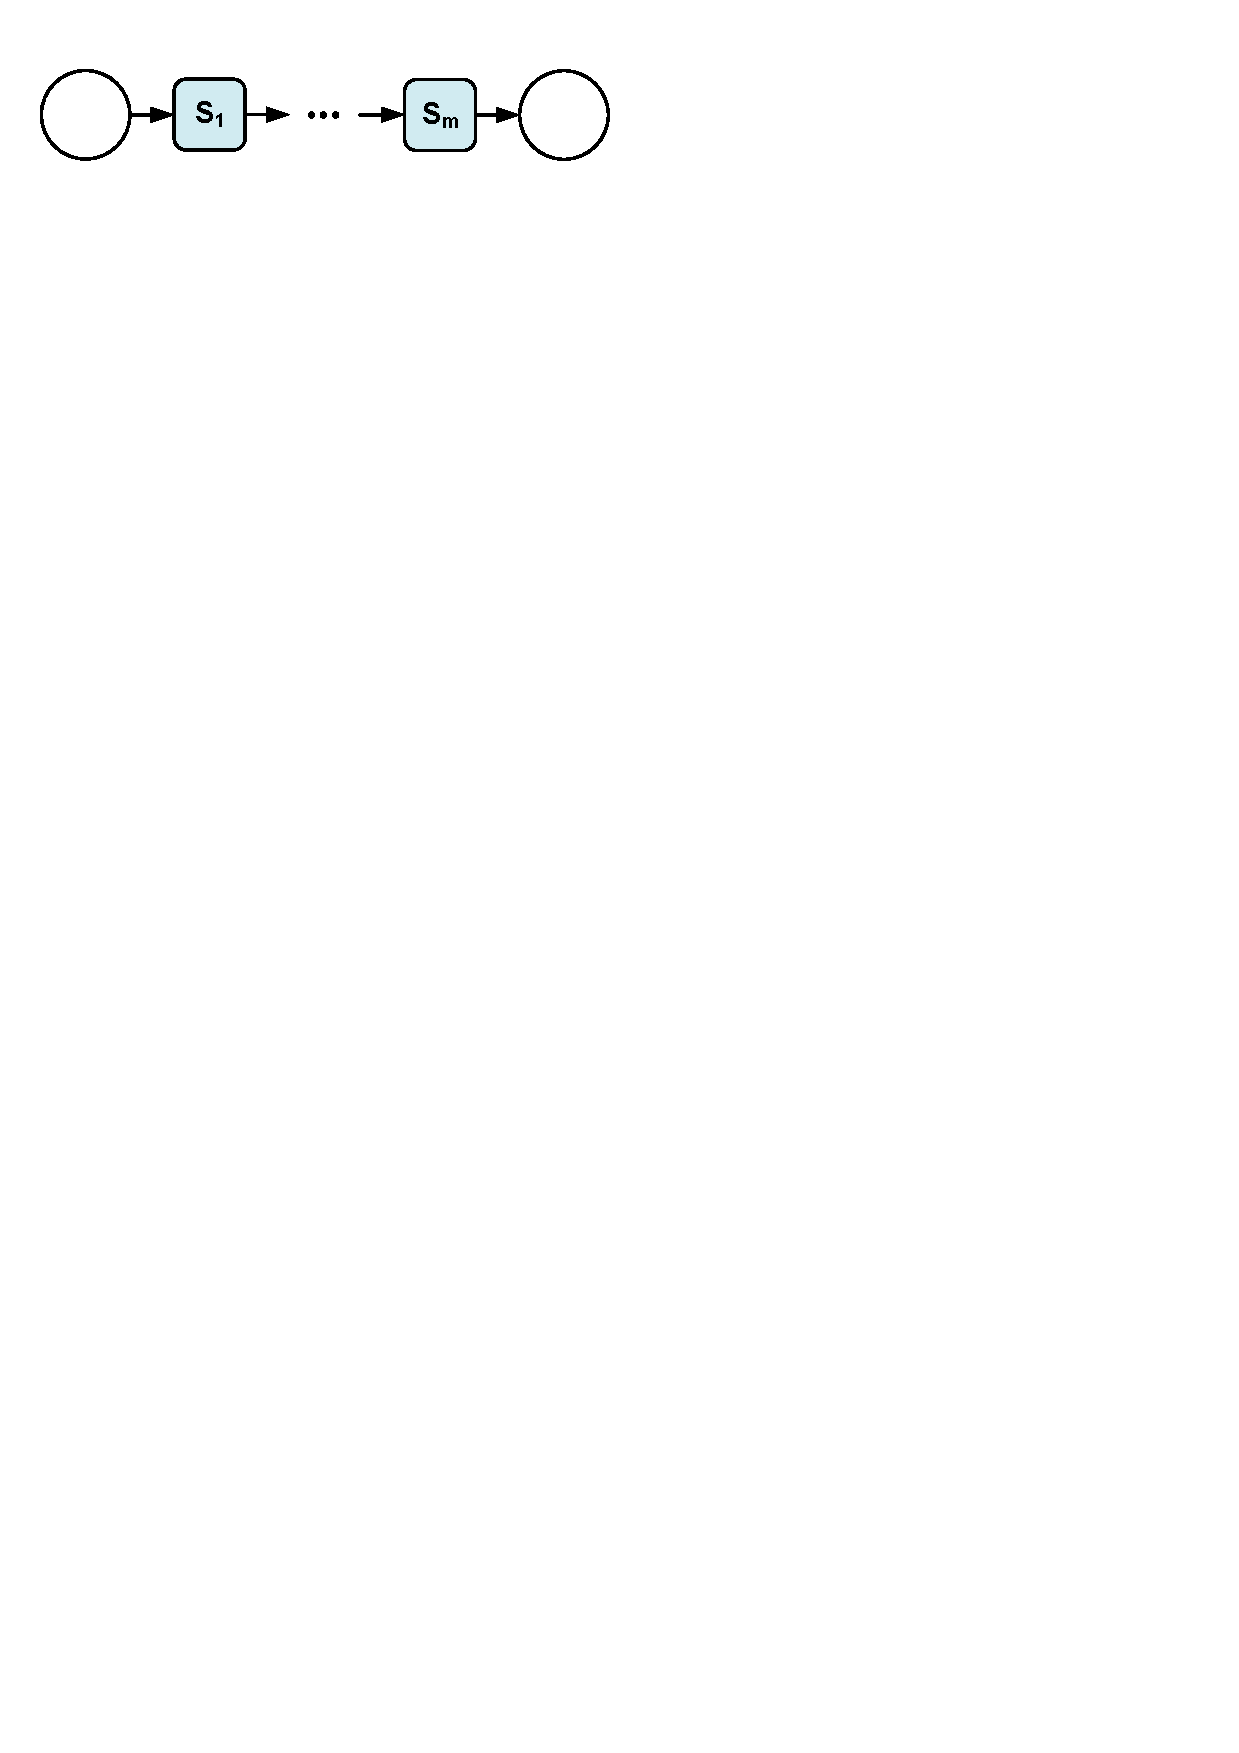
\includegraphics[width=1.4in]{sequence.pdf}\hfill\space\\[0.2cm]
$T=\frac{\sum\limits^m_{n=1}t_n}{m}$ \hfill $C=\frac{\sum\limits^m_{n=1}c_n}{m}$ \hfill
$A=\prod\limits^m_{n=1}a_n$\\
\space\hfill $R=\prod\limits^m_{n=1}r_n$\hfill\space\\[0.2cm]
\end{tabular}}}
\caption{Sequence construct and calculation of its QoS properties.}
\label{fig:sequence}
\vspace{0.3cm}

\centerline{
\fbox{
\begin{tabular}{p{0.5\linewidth}}
\space\hfill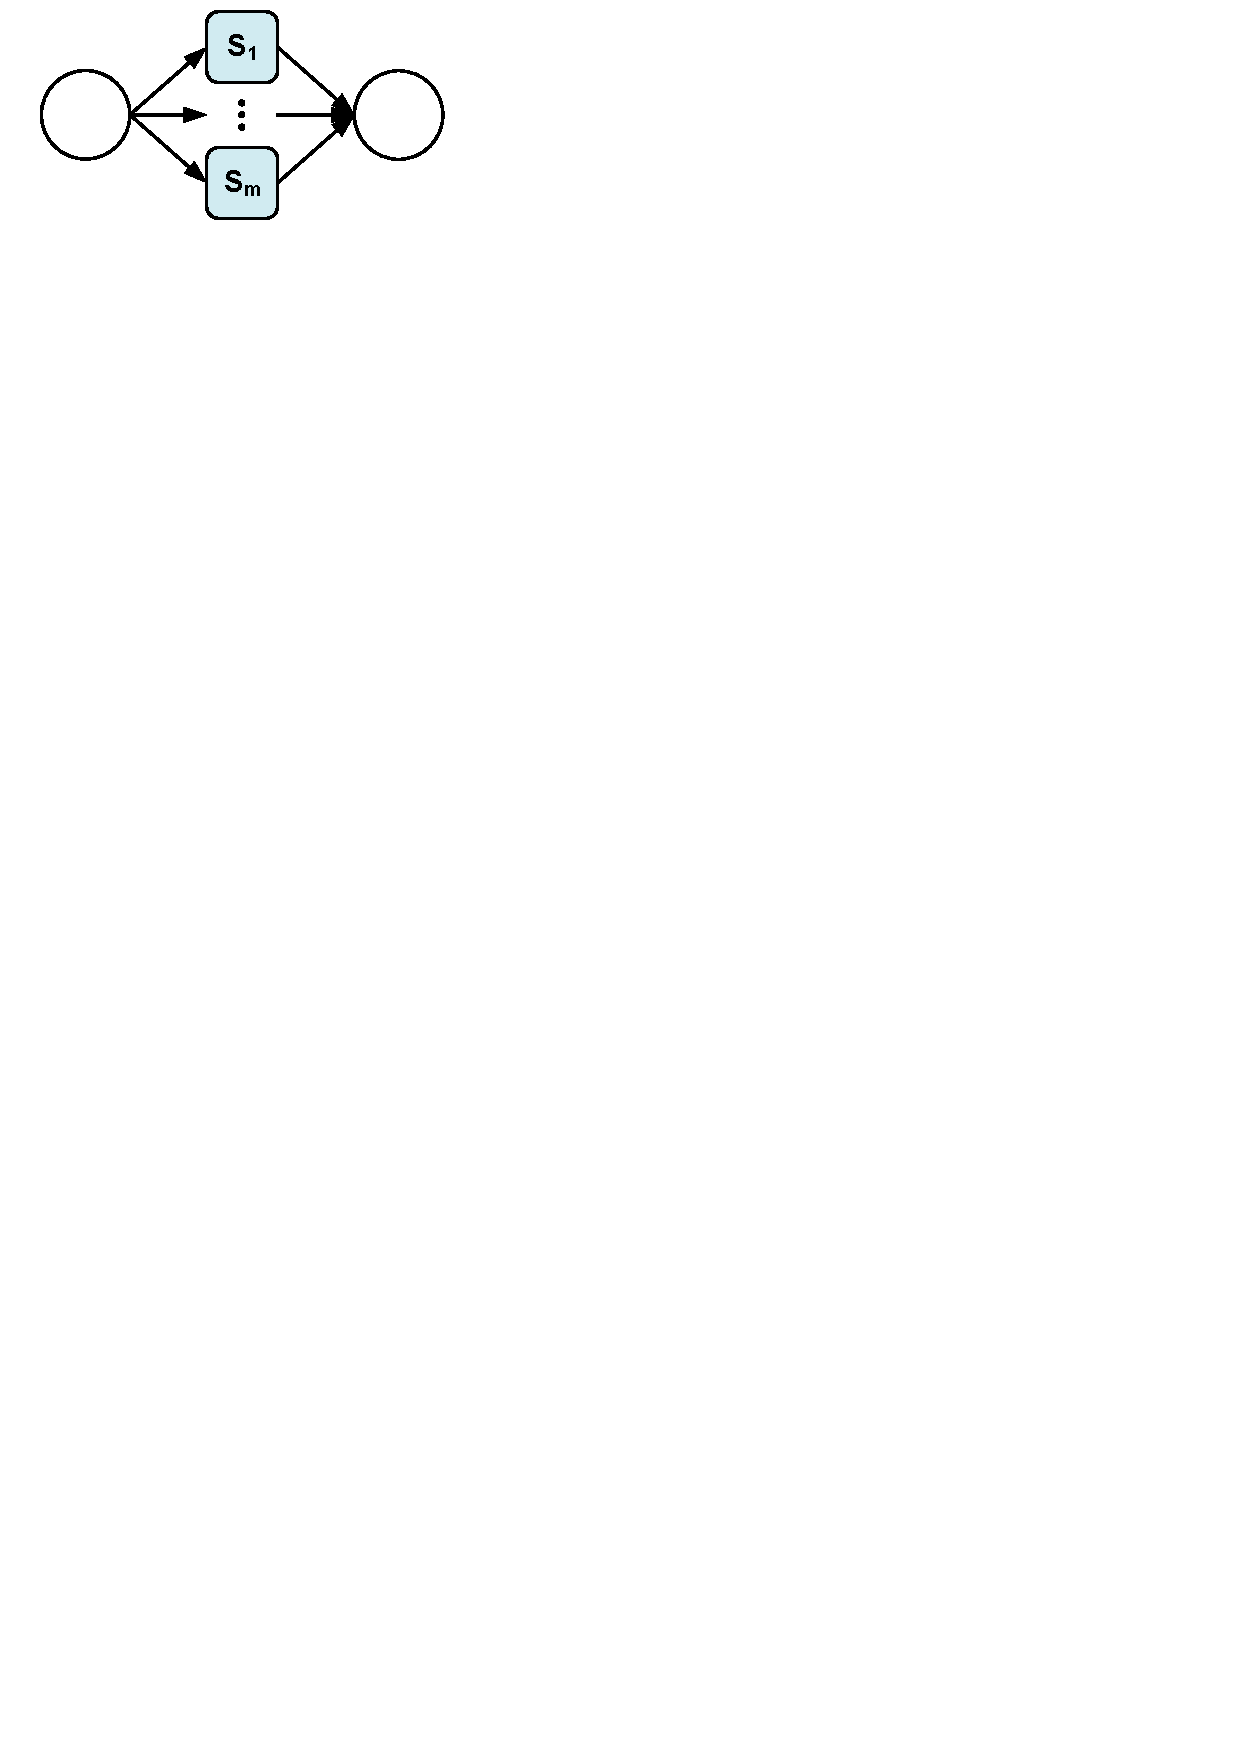
\includegraphics[width=1in]{parallel.pdf}\hfill\space\\[0.2cm]
\space\hfill$T=MAX\{t_n|n\in\{1,\ldots,m\}\}$\hfill\space\\[0.2cm]
$C=\frac{\sum\limits^m_{n=1}c_n}{m}$ \hfill $A=\prod\limits^m_{n=1}a_n$ \hfill
$R=\prod\limits^m_{n=1}r_n$
\end{tabular}}}
\caption{Parallel construct and calculation of its QoS properties.}
\label{fig:parallel}
\vspace{0.3cm}

\centerline{
\fbox{
\begin{tabular}{p{0.5\linewidth}}
\space\hfill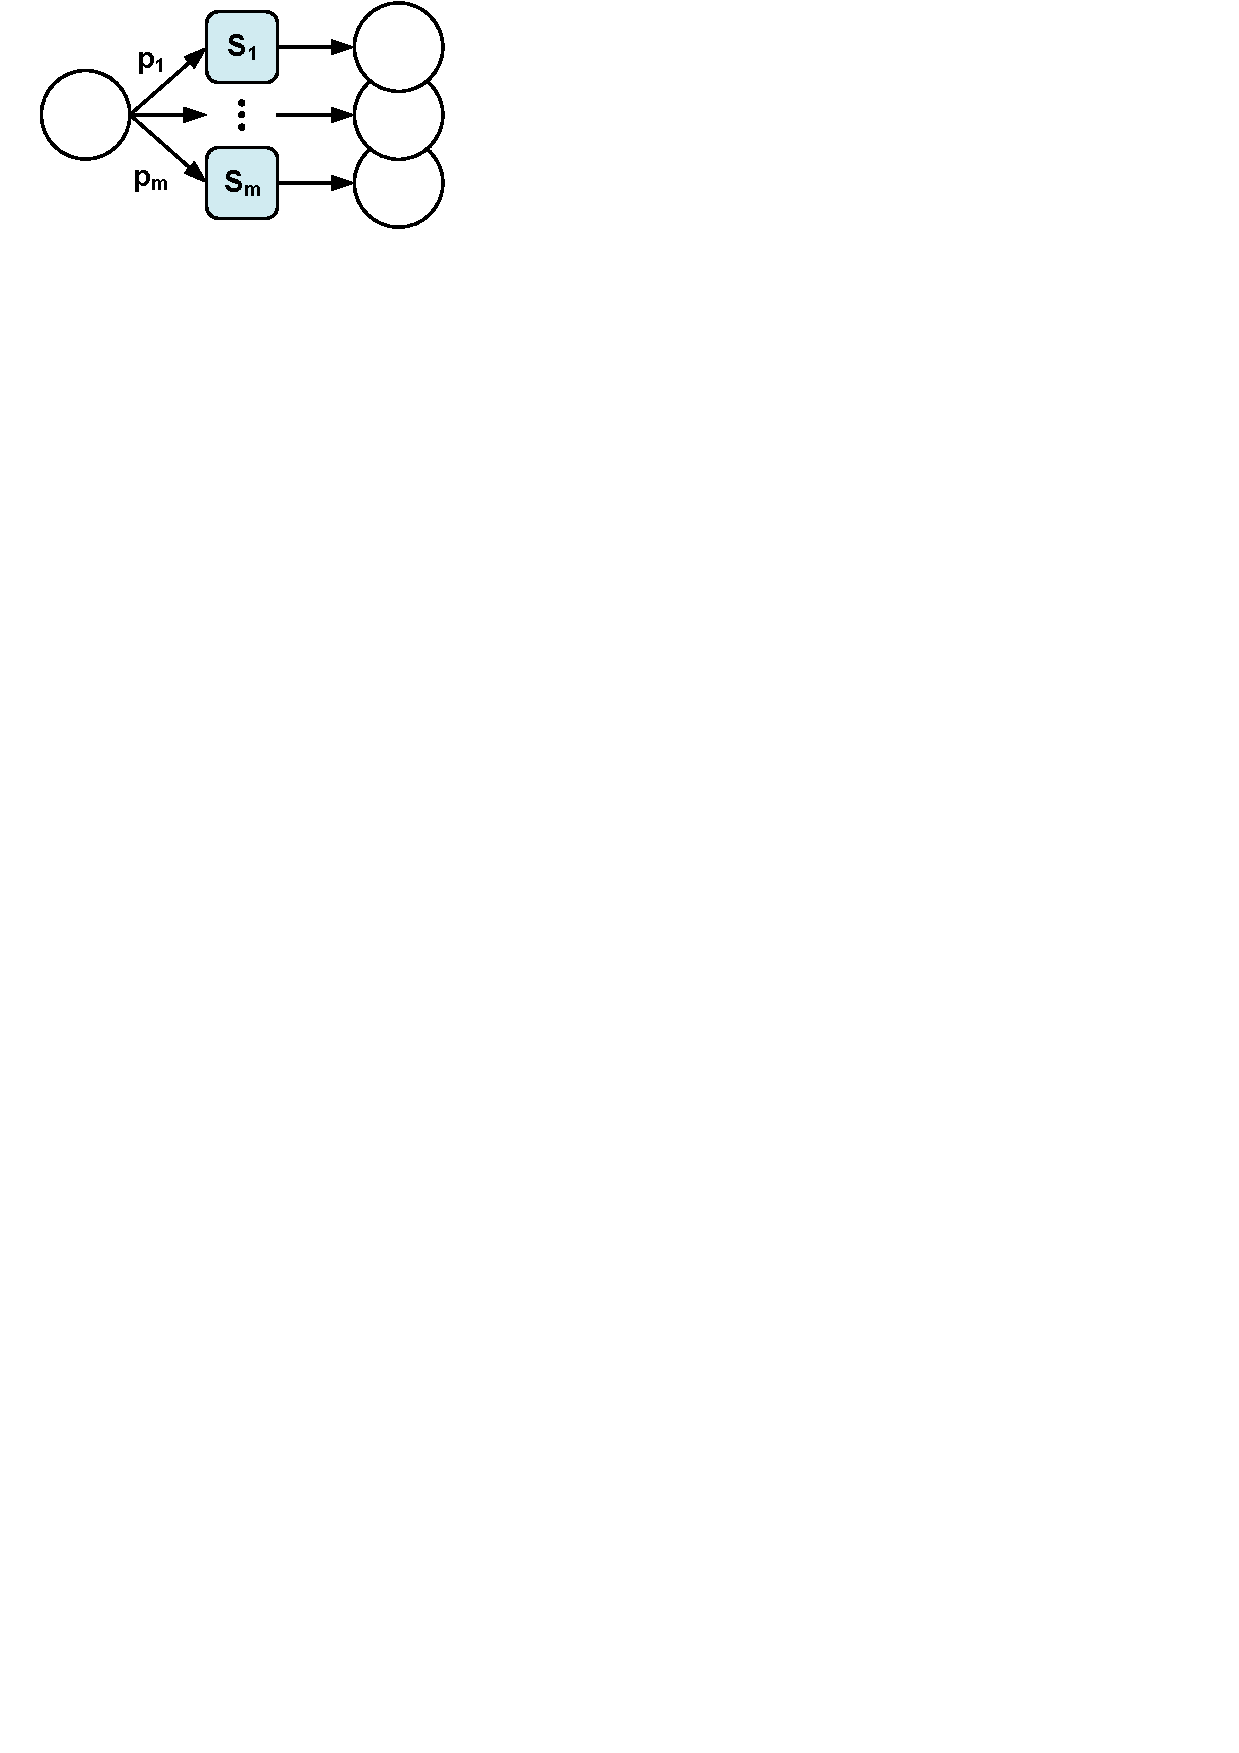
\includegraphics[width=1in]{conditional.pdf}\hfill\space\\[0.2cm]
$T=\sum\limits^m_{n=1}p_{n} t_{n}$ \hfill $C=\sum\limits^m_{n=1}p_{n} c_{n}$\hfill
$A=\sum\limits^m_{n=1}p_{n} a_{n}$\\
\space\hfill$R=\sum\limits^m_{n=1}p_{n} r_{n}$\hfill\space\\[0.2cm]
\end{tabular}}}
\caption{Choice construct and calculation of its QoS properties.}
\label{fig:conditional}
\end{figure}

\section{Fitness Function}
In EC-based composition approaches, the fitness function is used for optimising solutions according to their overall Quality of Service (QoS), and was based on the function shown in \cite{sawczuk2015gp}. This function measures the overall quality of a composition candidate by performing a weighted sum of the overall QoS attributes of a given candidate:

\begin{equation}
 fitness_i = w_1A_i + w_2R_i + w_3(1 - T_i) + w_4(1 - C_i)
\end{equation}

where $\sum_{i=1}^4{w_i} = 1$ \\

This function produces values in the range [0,1], where a fitness of 1 means the best possible quality, and a fitness of 0 means the worst. Because this is a maximising function, the Time $T$ and cost $C$ are offset by 1 in the formula, so that higher scores correspond to better qualities for these attributes as well. The overall quality attributes $A$, $R$, $T$, and $C$ of a composition are calculated according to formulae shown in Figures \ref{fig:sequence}, \ref{fig:parallel}, and \ref{fig:conditional}, and these values are then normalised to fit within the [0,1] range, according to Formulae \ref{availNormalise}, \ref{reliaNormalise}, \ref{timeNormalise}, and \ref{costNormalise}. These formulae are inspired by the work in \cite{ma2015hybrid}, and normalise the original overall composition values ($A_{orig}$, $R_{orig}$, $T_{orig}$, $C_{orig}$) by using the overall minimum and maximum values for each quality attribute over the entire service repository. In the formulae for calculating $T_i$ and $C_i$ the maximum values are multiplied by the total number $n$ of services in the repository, thus creating an upper bound for the normalisation. This is because a composition including all available candidate services would have the worst possible time and cost attributes.

\begin{equation}
A_i = \begin{cases}
     \frac{A_{orig} - A_{min}}{A_{max} - A_{min}}, & \text{ if }A_{max} - A_{min} \neq 0.\\
     1 & \mathrm{ otherwise}.
    \end{cases}
 \label{availNormalise}
\end{equation}

\begin{equation}
R_i = \begin{cases}
     \frac{R_{orig} - R_{min}}{R_{max} - R_{min}}, & \text{ if }R_{max} - R_{min} \neq 0.\\
     1 & \mathrm{ otherwise}.
    \end{cases}
 \label{reliaNormalise}
\end{equation}

\begin{equation}
T_i = \begin{cases}
     \frac{T_{orig} - T_{min}}{nT_{max} - T_{min}}, & \text{ if }nT_{max} - T_{min} \neq 0.\\
     0 & \text{ otherwise}.
    \end{cases}
 \label{timeNormalise}
\end{equation}

\begin{equation}
C_i = \begin{cases}
     \frac{C_{orig} - C_{min}}{nC_{max} - C_{min}}, & \text{ if }nC_{max} - C_{min} \neq 0.\\
     0 & \text{ otherwise}.
    \end{cases}
 \label{costNormalise}
\end{equation}

\section{Conditional Tree Representation}

The composition approach initially investigated employs Genetic Programming to evolve solutions according to their overall Quality of Service, meanwhile maintaining their functional correctness. A candidate solution for a composition is represented as a tree, where the non-terminal nodes represent the composition flow constructs (sequence, parallel, and conditional), and the terminal (leaf) nodes represent the atomic Web services included in the composition. An example of such a tree is shown in Figure \ref{fig:tree}. To calculate the overall QoS of a tree, the formulae in Figures \ref{fig:sequence}, \ref{fig:parallel} and \ref{fig:conditional} are employed, where the children of a current node act as the services used in the calculations. For Figure \ref{fig:tree}, for example, the QoS is first calculated for the sequence nodes directly above the leaves, then for the conditional node, and finally for the root node.

\begin{figure}
\centerline{
\fbox{
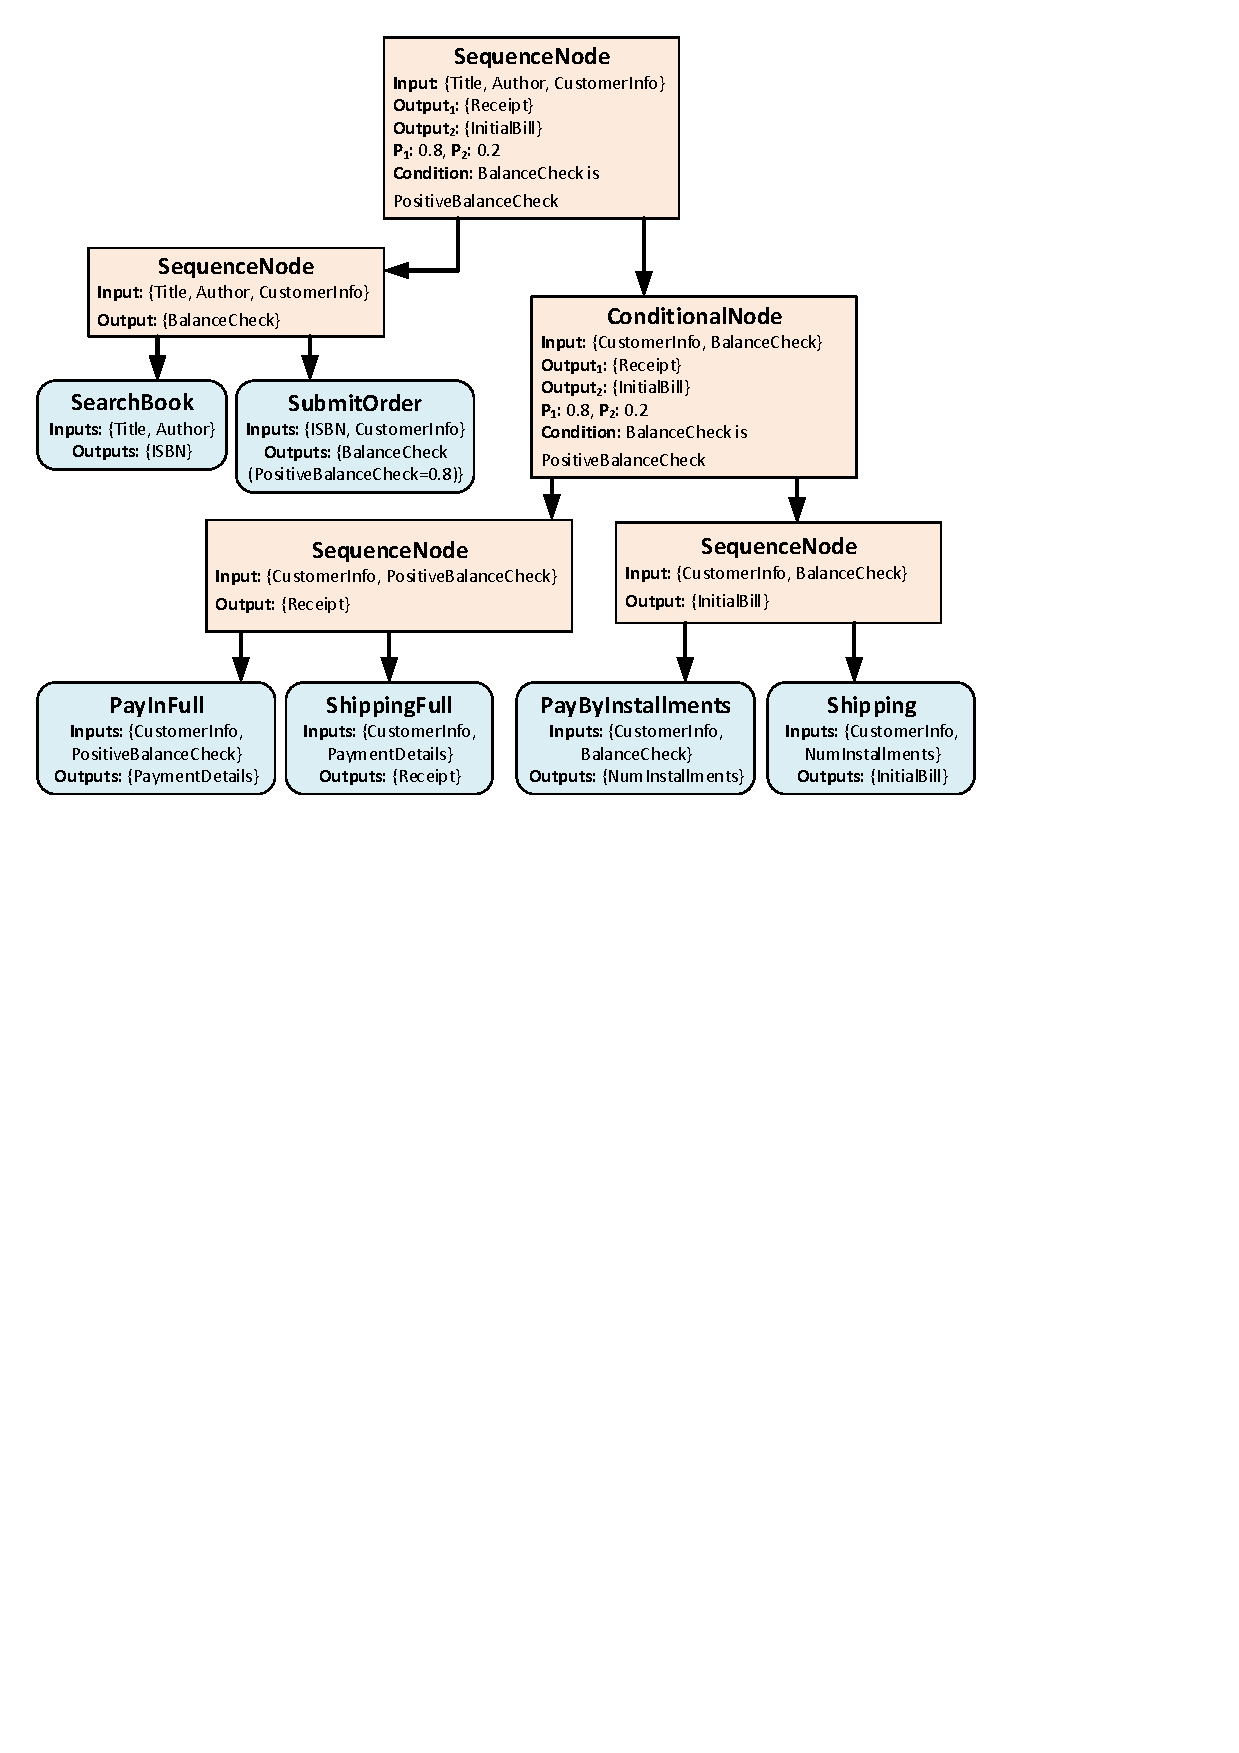
\includegraphics[width=8.4cm]{tree.pdf}
}}
\caption{Example of tree representation for Web service composition.}
\label{fig:tree}
\end{figure}

A population initialisation algorithm similar to the one in \cite{wang2013genetic} is employed, and so are constrained mutation and crossover operations. However, the difference of the current approach in comparison to \cite{wang2013genetic} is that it also considers the case where a user requires a conditional constraint to be met. The presence of conditional constraints means that different values are produced by a service at runtime, and these concrete values are subtypes of a statically defined concept. For example, a service that statically outputs a \textit{fruit} concept may output the subtype \textit{banana} at runtime, and thus conditions may be defined based on the different kinds of fruits. The relationship between types is held by a taxonomy that encodes the inputs and outputs pertinent to the candidate atomic services employed in the composition. For simplicity, the implementation presented in this work handles conditional constraints with two options (if and else), so this scenario will be the focus throughout the following sections.

\subsection{Population Initialisation}\label{init}
As opposed to generating a composition candidate purely based on a set of available inputs and another of desired outputs, we must also handle conditional constraints. A composition task with conditional constraints must include a set of available inputs, a condition of the is-a kind (e.g. if \textit{banana} $\succeq$ \textit{fruit}), and two sets of outputs, one expected in case the condition is met and the other in case it is not. With this information it is possible to run the initialisation algorithm and create a composition candidate in a graph format, later translated into a tree representation.

\begin{algorithm}
 \setlength\hsize{0.9\linewidth}
 \SetKwInOut{Input}{Input}\SetKwInOut{Output}{Output}
 \SetKwFunction{createGraph}{createGraph}\SetKwFunction{toTree}{toTree}
 \LinesNumbered
 \SetNlSty{}{}{:}
 \Input{$I$, $O_1$, $O_2$, $C$, $P$}
 \Output{candidate tree $T$}
 \eIf{$O_2 \neq \emptyset$}{
  $G_1 \leftarrow \createGraph(I \cup C.if, O_1)$\;
  $G_2 \leftarrow \createGraph(I \cup C.else, O_2)$\;
  $T_1 \leftarrow \toTree(G_1.input)$\;
  $T_2 \leftarrow \toTree(G_2.input)$\;
  $T_3 \leftarrow$ new $ConditionalNode$($C$)\;
  $T_3.leftChild \leftarrow T_1$\;
  $T_3.rightChild \leftarrow T_2$\;
  \eIf{$C \sqsubseteq I$}{
    $T_3.prob \leftarrow P$\;
    \KwRet $T_3$\;
  }{
    $G_4 \leftarrow \createGraph(I, C.else)$\;
    $T_4 \leftarrow \toTree(G_4.input)$\;
    $T_3.prob \leftarrow T_4.final.P$\;
    $T \leftarrow$ new $SequenceNode$()\;
    $T.leftChild \leftarrow T_4$\;
    $T.rightChild \leftarrow T_3$\;
    \KwRet $T$\;
  }
 }{
  $G \leftarrow \createGraph(I, O_1)$\;
  $T \leftarrow \toTree(G.input)$\;
  \KwRet $T$\;
 }
 \vspace{2mm}
 \caption{\footnotesize Generating a new candidate tree or a mutated subtree.}
\label{generation}
\end{algorithm}

Algorithm \ref{generation} is used to create a candidate which may incorporate a conditional constraint, though it is also capable of handling unconditional tasks. It requires a
set of inputs $I$, an if-else condition $C$, two sets of outputs $O_1$ (for if-branch) and $O_2$ (for else-branch). The set of probabilities $P$ is only required for a specific case, explained below, and $C$ as well as $O_2$ are not required for tasks without branching. The intuition behind this algorithm is to assemble a candidate tree in parts. Firstly, if the task has in fact two sets of outputs and a condition $C$, then two sub-composition graphs $G_1$ and $G_2$ are generated to represent the if and the else branches, respectively. This generation is performed using the $createGraph$ algorithm proposed in \cite{wang2013genetic}. Subsequently, these graphs are translated to trees $T_1$ and $T_2$ using the $toTree$ procedure proposed in Algorithm \ref{toTree}, and included as children of a $ConditionalNode$ created for condition $C$ (the left child represent the if-branch, and the right child the else-branch).

\begin{algorithm}
 \setlength\hsize{0.9\linewidth}
 \SetKwInOut{Input}{Input}\SetKwInOut{Output}{Output}
 \SetKwFunction{createParallelNode}{createParallelNode}\SetKwFunction{toTree}{toTree}
 \SetKwProg{Procedure}{Procedure}{}{}
 \LinesNumbered
 \SetNlSty{}{}{:}
 \Procedure{\toTree{}}{
 \Input{$N$}
 \Output{tree $T$}
 \uIf{$N$ is leaf}{
  \KwRet $N$\;
  }
  \uElseIf{$N = input$}{
    \eIf{$|N.to| = 1$}{
      $T \leftarrow \toTree(next.to[0])$\;
    }{
      $T \leftarrow \createParallelNode(N.to)$\;
    }
  }
  \uElse{
    $r$\;
    $children \leftarrow N.to - output$\;
    \eIf{$|children| = 1$}{
      $r \leftarrow \toTree(children[0])$\;
    }{
      $r \leftarrow \createParallelNode(children)$\;
    }
    $T \leftarrow$ new $SequenceNode$()\;
    $T.leftChild \leftarrow N$\;
    $T.rightChild \leftarrow r$\;
  }
  \KwRet $T$\;
  }
 \Procedure{\createParallelNode{}}{
 \Input{$children$}
 \Output{tree $T$}
 $T \leftarrow$ new $ParallelNode$()\;
 $subtrees \leftarrow \{\}$\;
 \ForEach{$c$ in $children$}{
    $S \leftarrow\toTree(c)$\;
    $subtrees \leftarrow subtrees \cup \{S\}$\;
 }
 $T.children \leftarrow subtrees$\;
 \KwRet $T$\;
 }
 \vspace{2mm}
 \caption{\footnotesize Converting graph into tree representation.}
\label{toTree}
\end{algorithm} 

Secondly, the algorithm verifies whether the value used for condition $C$ can be met by using the set of inputs $I$. If it can, then the set of probabilities $P$ of each branch being executed is associated to the $ConditionalNode$ and the tree is returned (this assumes that the probabilities for obtaining a specific value for the if condition in $C$ are already known -- typically during mutation). If it cannot, then another sub-composition graph $G_4$ is generated and translated to $T_4$, creating the part of the composition that leads from the available inputs $I$ to the value used in condition $C$. In this case, the probability associated with each branch of the condition is extracted from the last service in $T_4$ (i.e. the service that produces the overall sub-composition output that satisfies the value used in condition $C$), and a $SequenceNode$ is created as the tree root to link this deterministic part of the composition ($T_4$) to the conditional part ($T_3$). Finally, if no condition $C$ and output set $O_2$ are provided, then the candidate is generated purely by using the $createGraph$ and $toTree$ algorithms. 

For reasons of brevity, the $toTree$ procedure shown in Algorithm \ref{toTree} for converting a graph representation of a composition to a tree representation is not explained in detail. Its general idea is the same as the one discussed in \cite{nguyen2005text}, which is to recursively traverse a graph, starting from the start ($input$) node and working towards the end ($output$) node. At each node, the number of outgoing edges determines whether to create a sequential or a parallel construct, and $toTree$ recurses on each of the destination nodes of these outgoing edges. It is important to note that after creating the candidate tree, it must be traversed to determine the input values required to execute each node of the tree, and the output values produced by each node. This information is recorded within each node.

\subsection{Mutation and Crossover}\label{mutation}

The crossover operator employed in the evolutionary process swaps any two leaf nodes (i.e. Web services), one from each candidate, provided that these two leaves are functionally equivalent in terms of input and output values but represent different Web services. This particular crossover operation implementation was chosen because it provides an effective mechanism for performing Web service selection, whose objective is to identify the best service to perform a task out of a set of candidates providing the same functionality.
The mutation operator selects a node of the candidate tree at random, and using its input and output information produces a new subtree that may be structurally different yet provides the same functionality. The subtree is generated using Algorithm \ref{generation}, and is used to  replace the originally selected node in the candidate.

\section{Conditional Graph Representation}

The advantage of a tree representation is that its corresponding crossover and mutation operations are relatively simple to implement, since modifications are restricted to certain subtrees. However, both this approach presents the disadvantage of duplicating Web services throughout the tree, which means that modifying a part of the tree that contains a duplicated service may remove some fundamental connections to this service, thus breaking the correctness of the solution. Another disadvantage of this technique is that a graph representation must be generated first, and subsequently translated into a tree format, when attempting to generate trees with correct connections. These limitations can be addressed by representing solutions directly as graphs, since this data structure allows multiple output sets, does not require service node duplication, and does not need to be translated into another format after generation. However, genetic operations on graphs tend to be more complex, since they handle a greater number of node connections. A graph-based candidate may look like the representation shown in Figure \ref{fig:graph}, with each block encoded as a graph node, and edges flowing from the input (start) towards the output (end) nodes. Nodes with multiple children and/or multiple parents can also be included when necessary, meaning that Directed Acyclic Graphs (DAGs) are the basis of this representation.

\begin{figure}
\centerline{
\fbox{
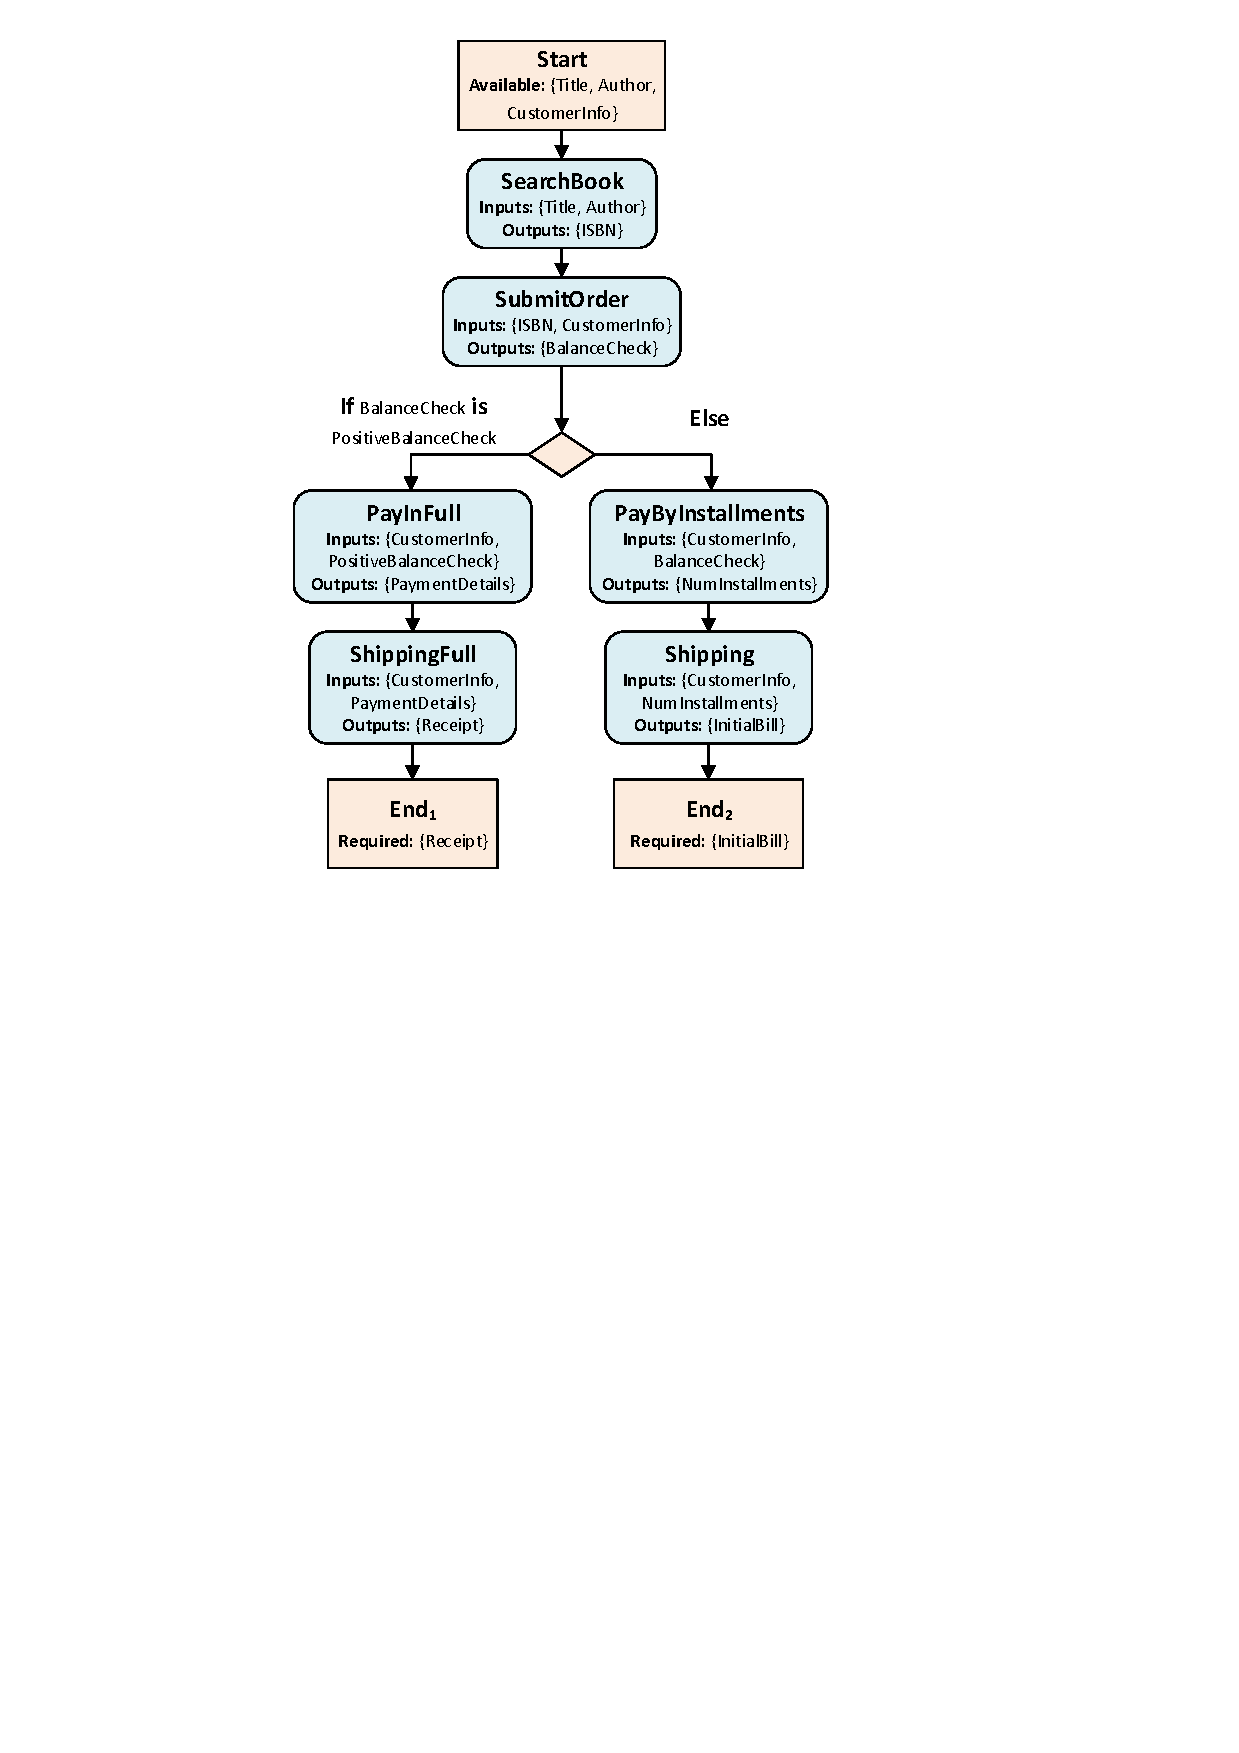
\includegraphics[width=6cm]{graph.pdf}
}}
\caption{Example of graph representation for Web service composition.}
\label{fig:graph}
\end{figure}

\subsection{Population Initialisation}

\begin{algorithm}
 \setlength\hsize{0.9\linewidth}
 \SetKwInOut{Input}{Input}\SetKwInOut{Output}{Output}
 \SetKwFunction{connectNode}{connectNode}\SetKwFunction{findCands}{findCands}\SetKwFunction{removeDangling}{removeDangling}\SetKwFunction{buildBranch}{buildBranch}
  \SetKwFunction{buildGraph}{buildGraph}\SetKwFunction{false}{false}\SetKwFunction{eNull}{null}
 \LinesNumbered
 \SetNlSty{}{}{:}
 %\Input{$InputNode$, $relevant$}
 %\Output{candidate graph $G$}
 
 \SetKwProg{myproc}{Procedure}{}{}
 \myproc{\buildGraph{$InputNode, relevant, candMap$}}{
 $start.outputs \leftarrow \{InputNode.values\}$\;
 $TaskNode \leftarrow InputNode.child$\;
 $G.edges \leftarrow \{\}$\;
 $G.nodes \leftarrow \{\}$\;
 $allInputs \leftarrow \{\}$\;
 $connections \leftarrow \{\}$\;
 \connectNode{$start,connections,G,allInputs,TaskNode$}\;
 $allowedAncestors \leftarrow \{start\}$\;
 \eIf{$candMap$ is \eNull}{
 $candList \leftarrow$ \findCands{$start,allowedAncestors,relevant$}\;
 }{
 $candList \leftarrow \{node | (start,node) \in candMap\}$\;
 }
 \buildBranch{$TaskNode,candList,connections,allInputs,G,$
 $relevant,allowedAncestors,candMap$}\;
 \removeDangling{$G$}\;
 \KwRet $G$\;
 }
 
 \vspace{2mm}
 \SetKwProg{myproc}{Procedure}{}{}
 \myproc{\connectNode{$n, connections, G, allInputs, TaskNode$}}{
  $n.objective \leftarrow TaskNode$\;
  $G.nodes \leftarrow G.nodes \cup \{n\}$\;
  $G.edges \leftarrow G.edges \cup connections$\;
  \eIf{$TaskNode$ is $ConditionNode$}{
    \eIf{$|n.outputs| > 1$}{
      \KwRet $((TaskNode.general \sqsubseteq n.outputs.general \wedge TaskNode.specific \sqsubseteq n.outputs.specific), n)$\;
    }{
      \KwRet $($\false$,n)$\;
    }
  }{
     \KwRet $(TaskNode.outputs \sqsubseteq allInputs, n)$\;
  }
}
 \caption{\footnotesize Procedures for building a new candidate graph and for connecting a particular node to the graph.}
\label{graph-generation}
\end{algorithm}

As with the fundamental GP technique, a graph-building algorithm is used to initialise the population of candidates so that the connections between the different atomic services included in a composition are correct. In this work, however, this algorithm is extended to create solutions with one input but multiple outputs, depending on the branching conditions specified. This extended version is shown in Algorithm \ref{graph-generation}.

Candidates are created using the $buildGraph$ procedure. This procedure requires $Input$ $Node$, which is the root of the composition's task tree, a list of $relevant$ candidate services from the service repository, and optionally a $candMap$. The $candMap$ is used for the crossover procedure only, so it will be discussed later. Given these inputs, the algorithm proceeds to connect nodes to the graph, one at a time, until a complete solution is found. As explained earlier, the resulting composition will have several independent branches, thus the recursive procedure $buildBranch$ has been created to handle each part of the composition. After connecting the $start$ node to the graph, we execute $buildBranch$ providing the first task it should achieve (i.e. $TaskNode$, which initially will be a conditional branching node), a list of candidates $candList$ that contains services that are executable/reachable using the $start$ node outputs, the partially built graph $G$, and other relevant data structures. Once the $buildBranch$ procedure has finished executing, the graph $G$ will be completed. The algorithm used for construction creates graphs from the $start$ node to the $end$ nodes in order to prevent cycles from forming, but this may lead to \textit{dangling} nodes, which are nodes that do not have any outgoing edges despite not being $end$ nodes. These are redundant parts of the solution, and thus they must be removed once $G$ is built. Finally, the creation of the new candidate graph is finished.

Algorithm \ref{graph-generation} also describes the $connectNode$ procedure, used for adding a node to an existing graph. In addition to adding the given node $n$ to $G$, and connecting it using the edges provided in the $connections$ list, this procedure also checks if the current $TaskNode$ objective has been reached. If the $TaskNode$ represents a conditional node, we check that we are now capable of producing both the  values required by the \textit{if} case and by the \textit{else} case when using the service we have just connected. On the other hand, if the $TaskNode$ represents the $end$ of a branch, we check that the list $allInputs$ of potential inputs contain all values necessary to satisfy the inputs fo the $end$ node.

\begin{algorithm}
 \setlength\hsize{0.9\linewidth}
 \SetKwFunction{connectNode}{connectNode}\SetKwFunction{findCands}{findCands}\SetKwFunction{removeDangling}{removeDangling}\SetKwFunction{buildBranch}{buildBranch}
 \SetKwFunction{false}{false} \SetKwFunction{true}{true}\SetKwFunction{eNull}{null}\SetKwFunction{connectTaskNode}{connectTaskNode}
 \LinesNumbered
 \SetNlSty{}{}{:}

 \SetKwProg{myproc}{Procedure}{}{}
 \myproc{\buildBranch{$TaskNode,candList,allInputs,G,$\\
 $relevant,allowedAncestors,candMap$}}{
  $goalReached \leftarrow$ \false\;
  $connResult$\;
  \While{$\lnot goalReached$}{
  $found \leftarrow$ \false\;
   \ForEach{$cand \in candList$}{
    $connections \leftarrow \{\}$\;
    $ancestors \leftarrow \{x.outputs | x \in G \wedge x \in allowedAncestors\}$\;
    \If{$cand.inputs \sqsubseteq ancestors$}{
      $connections \leftarrow connections \cup \{x \leftarrow minimal(ancestors)\}$\;
      $found \leftarrow$ \true\;
    }
   
   \If{$found$}{
   	$connResult \leftarrow$ \connectNode{$cand,connections,G,allInputs,TaskNode$}\;
   	$goalReached \leftarrow connResult[0]$\;
   	$allowedAncestors \leftarrow allowedAncestors \cup \{cand\}$\;
   	\eIf{$candMap$ is \eNull}{
   	$candList \leftarrow candList \cup$ \findCands{$cand,allowedAncestors,relevant$}\;
   	}{
   	$candList \leftarrow candList \cup \{node | (cand,node) \in candMap\}$\;
   	}
   	break\;
   }
   }
     $candList \leftarrow candList - \{cand\}$
  }
  \connectTaskNode{$TaskNode,connResult,G,allowedAncestors,$
  $candList,candMap$}\;
  }
 \caption{\footnotesize Indirectly recursive procedure for building one of the branches of the new candidate graph.}
\label{recAlgo}
\end{algorithm}

Algorithm \ref{recAlgo} shows the $buildBranch$ procedure, which recursively creates the bran\-ched Web service composition. Given a $TaskNode$, this procedure repeatedly adds 
services to the graph $G$, until the $TaskNode$ goal has been reached. More specifically, nodes from the $candList$ are considered for addition. A candidate $cand$ is randomly chosen from $candList$, and it is connected to the graph (using the $connectNode$) procedure if all of its inputs can be fulfilled by the $ancestor$ outputs (i.e. the outputs of nodes already present in that particular execution branch). The set of services in $connections$, which are used to connect $cand$ to $G$, is a minimal set, meaning that the output of these services fulfils all the inputs of $cand$, but if any connection is removed from the set that is no longer the case. After each $cand$ service is connected to $G$, the $candList$ is updated to contain any services that have now become executable due to the outputs of $cand$, and to exclude $cand$. Once the $TaskNode$ goal has been reached, the $connectTaskNode$ procedure is called to finish the construction of that branch, either by connecting an $end$ node to it or by further splitting the branch according to a new $TaskNode$ condition. In case of the latter, $connectTaskNode$ will invoke the $buildBranch$ procedure again.

\begin{algorithm}
 \setlength\hsize{0.9\linewidth}
 \SetKwFunction{connectNode}{connectNode}\SetKwFunction{findCands}{findCands}\SetKwFunction{removeDangling}{removeDangling}\SetKwFunction{buildBranch}{buildBranch}
 \SetKwFunction{false}{false} \SetKwFunction{true}{true}\SetKwFunction{eNull}{null}\SetKwFunction{connectTaskNode}{connectTaskNode}
 \LinesNumbered
 \SetNlSty{}{}{:}

 \SetKwProg{myproc}{Procedure}{}{}
 \myproc{\connectTaskNode{$TaskNode,connResult,G,$
 $allowedAncestors,candList,candMap$}}{
  \eIf{$TaskNode$ is $ConditionalNode$}{
  	$TaskGoal.probs \leftarrow connResult[1].probs$\;
  	$G.nodes \leftarrow G.nodes \cup \{TaskNode\}$\;
  	$G.edges \leftarrow G.edges \cup \{connResult[1] \rightarrow TaskNode\}$\;
  	$allowedAncestors \leftarrow allowedAncestors \cup \{TaskNode\}$\;
  	$connections \leftarrow \{\}$\;
  	\eIf{$candMap$ is \eNull}{
	  $candList \leftarrow candList \cup$ \findCands{$TaskNode, allowedAncestors, relevant$}\;
  	}{
  	$candList \leftarrow candList \cup \{node | (TaskNode,node) \in candMap\}$\;
  	}
  	$allInputs \leftarrow \{\}$\;
  	$ifChild \leftarrow TaskNode.ifChild$\;
  	\If{$ifChild$ is $OutputNode$}{
	   $allInputs \leftarrow \{x.outputs | x \in allowedAncestors\}$\;  	
  	}
  	\buildBranch{$ifChild, candList, allInputs, G, relevant,$
  	$allowedAncestors,candMap$}\;
  	$elseChild \leftarrow TaskNode.elseChild$\;
  	\If{$elseChild$ is $OutputNode$}{
  		$allInputs \leftarrow \{x.outputs | x \in allowedAncestors\}$\;
  	}
  	\buildBranch{$elseChild, candList, allInputs, G, relevant,$
  	$allowedAncestors,candMap$}\;
  }{
  $ancestors \leftarrow \{x.outputs | x in G \wedge x \in allowedAncestors\}$\;
  $connections \leftarrow \{x \rightarrow TaskNode\ | x \in minimal(ancestors)\}$\;
  $G.nodes \leftarrow G.nodes \cup \{TaskNode\}$\;
  $G.edges \leftarrow G.edges \cup connections$\;
  }
  }
 \caption{\footnotesize Procedure for finishing construction of a branch, splitting it further in case another
 condition exists.}
\label{taskAlgo}
\end{algorithm}

As previously explained, Algorithm \ref{taskAlgo} is responsible for finishing the construction of a given execution branch, according to one of two scenarios. In the first scenario, the $TaskNode$ reached is a conditional node, meaning that the branch will be further split into an \textit{if-and-else} structure. In this case, the $TaskNode$ is added to $G$, connected through the previously added service in $connResult[1]$ (i.e. the service that fulfilled the outputs required for the condition to be checked). Whenever a branching node is added, probability values must be associated with each path, indicating the likelihood of that path being executed. Since the branching occurs based on the values produced by  
$connResult[1]$, the probabilities of producing these different output possibilities are copied from this service. Then, the $buildBranch$ procedure is invoked twice more, once for the $if$ branch and once for the $else$ branch, providing the appropriate children of $TaskNode$ to the next construction stages. In the second scenario, the $TaskNode$ reached is an output node, meaning that the branch leads to an $end$ node without any further splitting. In this case, the $TaskNode$ is simply connected to $G$, using a minimal set of services already in the graph which produce all the outputs required by this $end$ node.

\subsection{Mutation and Crossover}

\begin{algorithm}
 \setlength\hsize{0.9\linewidth}
 \SetKwFunction{connectNode}{connectNode}\SetKwFunction{findCands}{findCands}\SetKwFunction{removeDangling}{removeDangling}\SetKwFunction{buildBranch}{buildBranch}
 \SetKwFunction{false}{false} \SetKwFunction{true}{true}\SetKwFunction{eNull}{null}\SetKwFunction{connectTaskNode}{connectTaskNode}\SetKwFunction{mutation}{mutation}
 \SetKwFunction{crossover}{crossover}\SetKwFunction{selectNode}{selectNode} \SetKwFunction{removeNodes}{removeNodes}
 \LinesNumbered
 \SetNlSty{}{}{:}

 \SetKwProg{myproc}{Procedure}{}{}
 \myproc{\mutation{$G, InputNode, relevant$}}{
 $n \leftarrow$ \selectNode{$G$}\;
 \eIf{$n$ is $start$}{
  \KwRet \buildGraph{$InputNode, relevant,$ \eNull}\;
 }{
  $TaskNode \leftarrow n.objective$\;
  \removeNodes{$n$}\;
  $allInputs \leftarrow \{\}$\;
  $candList \leftarrow \{\}$\;
  $allowedAncestors \leftarrow \{\}$\;
  \ForEach{$node \in G.nodes$}{
    $allowedAncestors \leftarrow allowedAncestors \cup \{node\}$\;
  }
  \ForEach{$node \in G.nodes$}{
    $candList \leftarrow candList \cup$ \findCands{$node, allowedAncestors, relevant$}\;
  }
  \If{$TaskNode$ is $OutputNode$}{
    $allInputs \leftarrow \{x.outputs | x \in allowedAncestors\}$\;
  }
  \KwRet \buildBranch{$TaskNode, candList, allInputs, G, relevant,$
  $allowedAncestors,$\eNull}\;
 }
 }
 
  \myproc{\crossover{$G_1, G_2, InputNode, relevant$}}{
  $candMap \leftarrow \{(x,y) | x \rightarrow y \in G_1.edges\}$\;
  $candMap \leftarrow candMap \cup \{(x,y) | x \rightarrow y \in G_2.edges\}$\;
  \KwRet \buildGraph{$InputNode, relevant, candMap$}\;
  }
 
 \caption{\footnotesize Procedures for performing mutation and crossover on graph candidates.}
\label{operatorsAlgo}
\end{algorithm}

The procedures for performing the mutation and crossover operations are shown in Algorithm \ref{operatorsAlgo}. The general idea behind the $mutation$ procedure is to modify a part of the original graph $G$, but maintain the rest of the graph unchanged. In order to do so, a node $n$ is initially selected as the mutation point, provided that it is not an $end$ or a $condition$ node. If this node is the $start$ node, an entirely new candidate graph is constructed; otherwise, all nodes whose input satisfaction depends upon node $n$ are removed from $G$, and so are any subsequent splits of that branch. The construction of this partially-built graph is then finished by invoking the $buildBranch$ procedure and providing the original $TaskNode$ ($n$'s objective) and appropriate data structures to it. The $allowedAncestors$, the $candList$, and $allInputs$ are calculated based on the remaining nodes of $G$. The mutation operator was designed in this way so that it allows for variations of the original candidate, at the same time maintaining the correctness of the connections between services (nodes) in the graph.

In the case of $crossover$, the general idea is to reuse connection patterns from two existing candidates $G_1$ and $G_2$ in order to create a new child candidate that combines elements from these two parents. In order to do so, the original connections of $G_1$ and $G_2$ are abstracted into a map called $candMap$. This map can be queried to determine all the connections (from both parents) that can be made starting from a given node $x$, e.g. $x$ connects to $y_1$, $y_2$, and $y_3$ in $G_1$ and $G_2$. After having assembled this map, the $buildGraph$ procedure is invoked to create a child candidate. The difference is that the addition of candidates to the $candList$ is done by querying the $candMap$ to determine which services could be reached from the current node according to the connection patterns in the original parents. One of the advantages of this crossover implementation is that it allows for a flexible operation that reuses connection information from both parents. Additionally, this operation can be executed using the already existing graph-building algorithm with minimal changes.

\section{Experiment Design}\label{experimentDesign}
Experiments were conducted to compare the performance of the graph-based representation to that of the tree-based representation. The datasets employed in this comparison were based on those proposed in \cite{sawczuk2015gp}, since they contain composition tasks that require one conditional constraint. The initial sets were extended to make the problem more complex by replicating each original service ten times. The replicated services were then assigned randomly generated QoS values that were within the original ranges for each quality attribute. A new dataset, also based on those presented in \cite{sawczuk2015gp}, was created to measure the performance of our technique when addressing more complex composition tasks. In this case, the composition task has three conditional constraints. Because the tree approach cannot handle more than one conditional constraint, it has not been tested with this dataset.

\subsection{Parameters}
Tests were executed on a personal computer with an Intel Core i7-4770 CPU (3.4 GHz), and 8GB RAM. In total, four different tests were executed, three of them being comparisons and the fourth being an experiment on the behaviour of the graph approach only. The EC parameters used for these experiments are shown in Table \ref{tab:settings}. As it can be seen from the table, the parameters for the comparison were based on those proposed by Koza \cite{koza1992genetic}, with a mutation probability of 0.1 (instead of Koza's 0.0) so that the mutation operators could also be tested. Results were calculated out of 30 independent runs for all four tests. Finally, all fitness function weights were set to 0.25, indicating that all quality attributes are considered equally important by the user requesting the composition.

\begin{table}
\fontsize{7}{7}\selectfont\sffamily

\centerline{
\def\arraystretch{1.5}
\begin{tabular}{l|c|}
\cline{2-2}
                                                        & \multicolumn{1}{l|}{\textbf{All experiments}} \\ \hline
\multicolumn{1}{|l|}{\textbf{Independent runs}}         & 30                                            \\ \hline
\multicolumn{1}{|l|}{\textbf{Population size}}          & 500                                           \\ \hline
\multicolumn{1}{|l|}{\textbf{Generations}}              & 51                                            \\ \hline
\multicolumn{1}{|l|}{\textbf{Crossover probability}}    & 0.8                                           \\ \hline
\multicolumn{1}{|l|}{\textbf{Mutation probability}}     & 0.1                                           \\ \hline
\multicolumn{1}{|l|}{\textbf{Reproduction probability}} & 0.1                                           \\ \hline
\multicolumn{1}{|l|}{\textbf{Elitism candidates}}       & 0                                             \\ \hline
\multicolumn{1}{|l|}{\textbf{Tournament size}}          & 2                                             \\ \hline
\multicolumn{1}{|l|}{\textbf{Fitness weights}}          & 0.25 (all)                                    \\ \hline
\end{tabular}
}
\vspace{0.2cm}
\normalfont
\caption{Experiment settings.}
\label{tab:settings}
\end{table}

\section{Results}\label{results}

The results have been organised into two subsections, one discussing the comparison between the two techniques when using the datasets whose tasks require one conditional constraint, and the other addressing the convergence behaviour of the graph-based technique when using the dataset whose task requires multiple conditional constraints.

\subsection{Comparison Tests}

The results of the comparison between the two composition techniques is shown in Table \ref{tab:comparison}, where the first column lists the dataset used and its number of services, the second column displays the mean time with standard deviation for executing the graph-based approach, the third column shows the mean fitness and standard deviation of the best solution found by the graph-based approach, and the fourth and fifth columns show the corresponding time and fitness values for the tree-based approach. Time values, including their standard deviations, are rounded to 1 decimal point of precision; fitness values and their standard deviations are rounded to 2 decimal points. Wilcoxon signed-ranked tests at 95\% confidence level were run where possible to ascertain whether there the differences in time and fitness values for a given dataset are significant, with $\downarrow$ denoting significantly lower values and $\uparrow$ denoting significantly higher values. The individual values used to calculate the mean time and mean fitness values shown in the table have also been plotted in Figures \ref{fig:time} and \ref{fig:fitness}, respectively.

\begin{table}

\fontsize{7}{7}\selectfont\sffamily
\centerline{
\def\arraystretch{1.5}
\begin{tabular}{c|c|c|c|c|}
\cline{2-5}
\multicolumn{1}{l|}{}                     & \multicolumn{2}{c|}{\textbf{Graph-based}}              & \multicolumn{2}{c|}{\textbf{Tree-based}}          \\ \hline
\multicolumn{1}{|c|}{\textbf{Set (size)}} & \textbf{Avg. time (s)}      & \textbf{Avg. fitness}    & \textbf{Avg. time (s)} & \textbf{Avg. fitness}    \\ \hline
\multicolumn{1}{|c|}{$1 (1738)$}          & $11.2 \pm 1.5 \downarrow$   & $0.76 \pm 0.02$          & $235.2 \pm 52.8$       & $0.85 \pm 0.01$          \\ \hline
\multicolumn{1}{|c|}{$2 (6138)$}          & $35.0 \pm 3.3 \downarrow$   & $0.67 \pm 0.01$          & $609.3 \pm 112.7$      & $0.65 \pm 0.00$          \\ \hline
\multicolumn{1}{|c|}{$3 (6644)$}          & $19.0 \pm 1.0 \downarrow$   & $0.72 \pm 0.01$          & $2264.5 \pm 296.2$     & $0.74 \pm 0.02$          \\ \hline
\multicolumn{1}{|c|}{$4 (11451)$}         & $49.1 \pm 1.6 \downarrow$   & $0.56 \pm 0.01$          & $900.6 \pm 138.2$      & $0.77 \pm 0.08 \uparrow$ \\ \hline
\multicolumn{1}{|c|}{$5 (11990)$}         & $34.9 \pm 1.3 \downarrow$   & $0.81 \pm 0.02$          & $2680.7 \pm 217.8$     & $0.83 \pm 0.01$          \\ \hline
\multicolumn{1}{|c|}{$6 (24178)$}         & $140.7 \pm 21.8 \downarrow$ & $0.77 \pm 0.02 \uparrow$ & $19772.2 \pm 2142.7$   & $0.76 \pm 0.02$          \\ \hline
\multicolumn{1}{|c|}{$7 (45243)$}         & $345.4 \pm 55.5 \downarrow$ & $0.79 \pm 0.02$          & $24467.1 \pm 5482.4$   & $0.90 \pm 0.03 \uparrow$ \\ \hline
\multicolumn{1}{|c|}{$8 (89309)$}         & $522.1 \pm 94.5 \downarrow$ & $0.82 \pm 0.00$          & $51850.3 \pm 5768.2$   & $0.82 \pm 0.04$          \\ \hline
\end{tabular}
}
\vspace{0.2cm}
\normalfont
\caption{Comparison results.}
\label{tab:comparison}
\end{table}

\begin{figure}
\centerline{
\fbox{
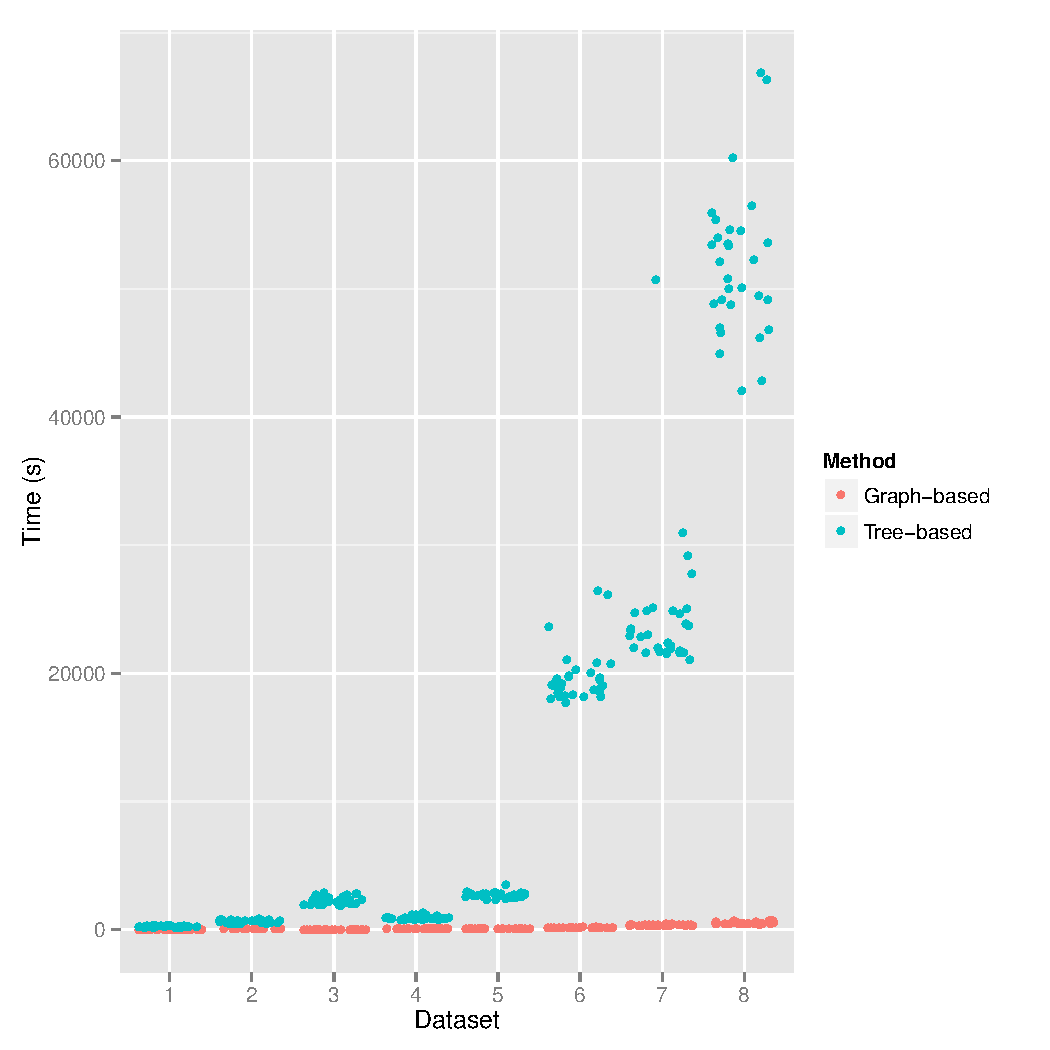
\includegraphics[width=8cm]{time.pdf}}}
\caption{Comparison of the execution time of both approaches for each dataset, over 30 independent runs.}
\label{fig:time}
\end{figure}

\begin{figure}
\centerline{
\fbox{
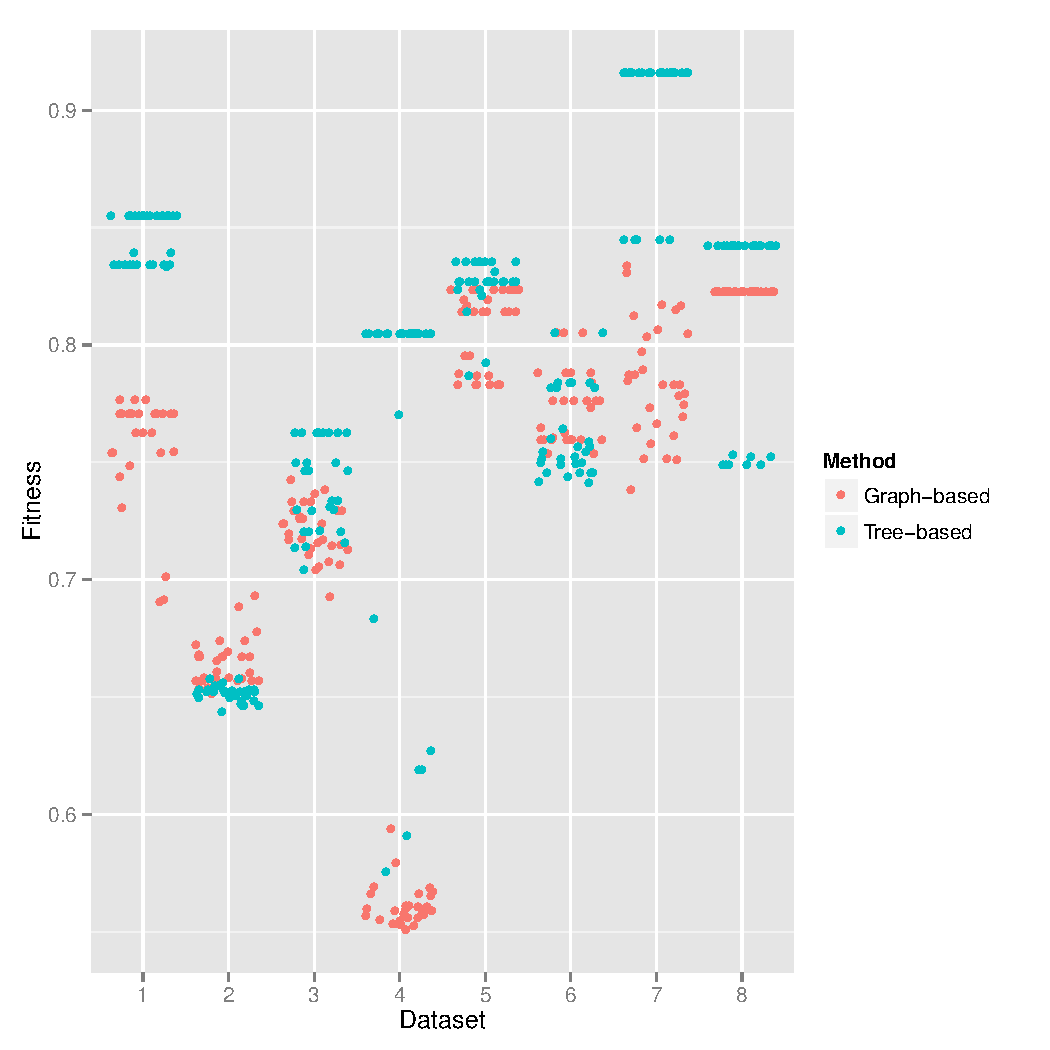
\includegraphics[width=8cm]{fitness.pdf}}}
\caption{Comparison of the best fitness of both approaches for each dataset, over 30 independent runs.}
\label{fig:fitness}
\end{figure}

As expected, the execution times of the graph-based approach are significantly lower than those of the tree-based approach for all datasets. Surprisingly, the performance gains of the graph-based method are more pronounced as the size of the dataset grows, culminating into a difference of two orders of magnitude for the largest dataset. These results are extremely encouraging, because they demonstrate that representing solutions directly as a DAG facilitates the enforcement of correct output-input connections between services, which in turn translates to lower execution costs. With regards to the quality of solutions, results show that the fitness is equivalent for the majority of datasets, but occasionally the quality of the solutions produced using the tree-based approach is superior. In particular, the tree fitness results for datasets 4 and 7 are significantly better than those produced by the graph-based approach, while the graph-based approach is significantly better for dataset 2. These results are mixed, indicating that the advantage of employing one approach over the other may change depending on the composition scenario, without clear superiority between them.

\subsection{Convergence Test}

\begin{figure}
\centerline{
\fbox{
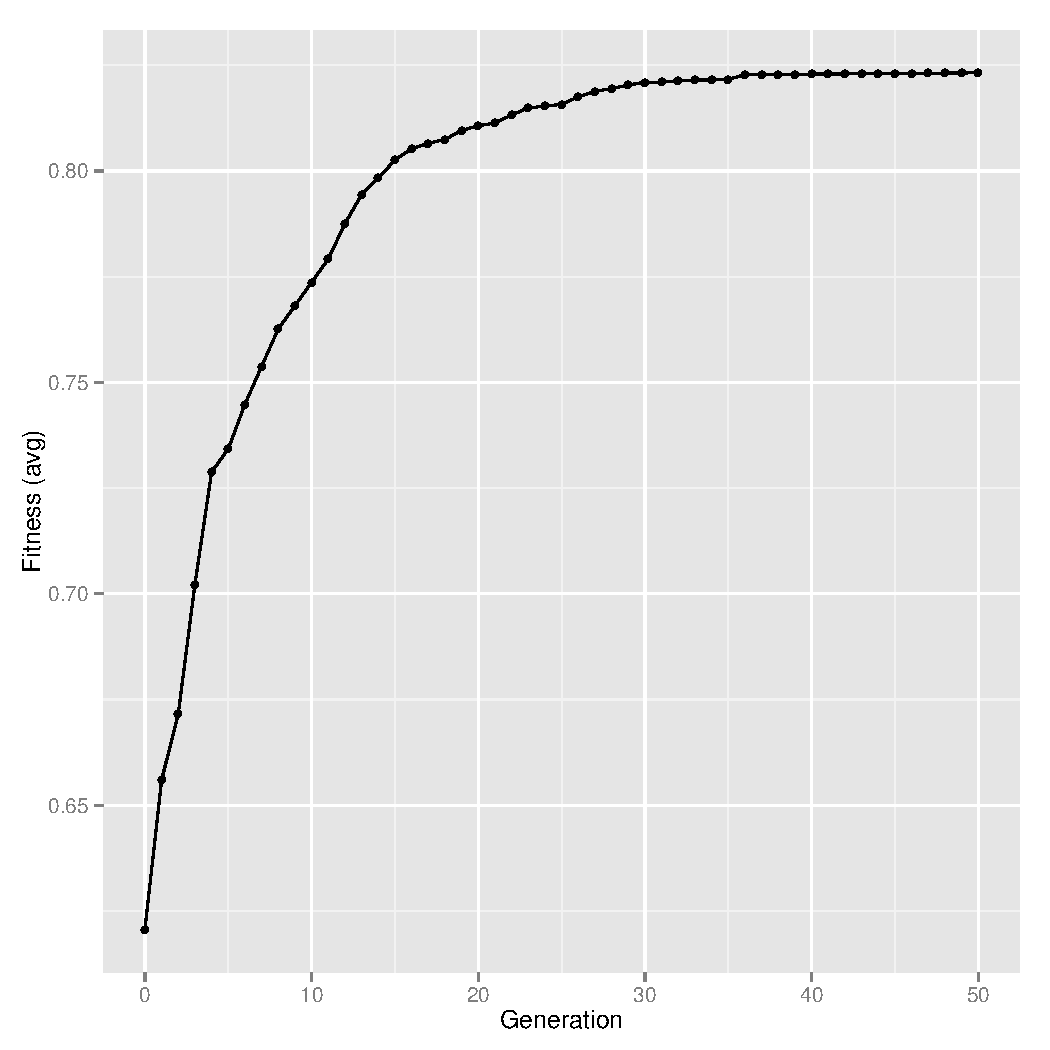
\includegraphics[width=8cm]{convergence.pdf}}}
\caption{Average fitness per generation with artificial optimum.}
\label{fig:convergence}
\end{figure}

The results of running the graph-based approach with the dataset that contains the artificial optimum are shown in Figure \ref{fig:convergence}, where the mean fitness values calculated over 30 independent runs have been plotted for each generation. The artificial optimum is known to correspond to the value $1$ when evaluated using the fitness function, which means that solutions with a value close to $1$ are likely to be close to this optimum. The plotted mean values clearly show that the most significant fitness improvements occur between generations 0 and  20-25, with the remaining generations performing smaller improvements that eventually lead to the convergence of the population. Interestingly, the fitness values between generations 40 and 50 remain constant at $0.88$, without the slightest variation. Upon closer inspection, it was found that all individual runs used when compiling this plot converge to a value of $0.88$, not progressing beyond this level. In some cases the fitness value of $0.88$ is reached by generation 25, but even then the population does not improve further in the remaining 25 generations. We hypothesise that this behaviour is caused by the genetic operators used in the graph-based approach, since the mutation and crossover patterns dictate the trajectory of the overall search. This suggests that improvements to these operators could be performed to improve the search strategies when using a DAG representation.
